\documentclass[sigplan,10pt,screen,anonymous]{acmart}
\renewcommand\footnotetextcopyrightpermission[1]{}

\settopmatter{printfolios=true,printacmref=false}

%%
%% \BibTeX command to typeset BibTeX logo in the docs
\AtBeginDocument{%
  \providecommand\BibTeX{{%
    Bib\TeX}}}

%% Rights management information.  This information is sent to you
%% when you complete the rights form.  These commands have SAMPLE
%% values in them; it is your responsibility as an author to replace
%% the commands and values with those provided to you when you
%% complete the rights form.
% \setcopyright{acmcopyright}
% \copyrightyear{2018}
% \acmYear{2018}
% \acmDOI{XXXXXXX.XXXXXXX}

%% These commands are for a PROCEEDINGS abstract or paper.
\acmConference[SOSP '23]{29th ACM Symposium on Operating Systems Principles}{October 23--26,
  2023}{Koblenz, Germany}
%%
%%  Uncomment \acmBooktitle if the title of the proceedings is different
%%  from ``Proceedings of ...''!
%%
%%\acmBooktitle{Woodstock '18: ACM Symposium on Neural Gaze Detection,
%%  June 03--05, 2018, Woodstock, NY}
% \acmPrice{15.00}
% \acmISBN{978-1-4503-XXXX-X/18/06}


%%
%% Submission ID.
%% Use this when submitting an article to a sponsored event. You'll
%% receive a unique submission ID from the organizers
%% of the event, and this ID should be used as the parameter to this command.
\acmSubmissionID{321}

%%
%% For managing citations, it is recommended to use bibliography
%% files in BibTeX format.
%%
%% You can then either use BibTeX with the ACM-Reference-Format style,
%% or BibLaTeX with the acmnumeric or acmauthoryear sytles, that include
%% support for advanced citation of software artefact from the
%% biblatex-software package, also separately available on CTAN.
%%
%% Look at the sample-*-biblatex.tex files for templates showcasing
%% the biblatex styles.
%%

%%
%% The majority of ACM publications use numbered citations and
%% references.  The command \citestyle{authoryear} switches to the
%% "author year" style.
%%
%% If you are preparing content for an event
%% sponsored by ACM SIGGRAPH, you must use the "author year" style of
%% citations and references.
%% Uncommenting
%% the next command will enable that style.
%%\citestyle{acmauthoryear}

% to be able to draw some self-contained figs
\usepackage{tikz}
\usepackage{amsmath}
\usepackage{grffile}

% inlined bib file
\usepackage{filecontents}
\usepackage{float}
\usepackage{graphicx}
\usepackage{subfig}
\usepackage[font=small,skip=1pt]{caption}

\usepackage{algpseudocode}
\usepackage[linesnumbered,ruled]{algorithm2e}
\usepackage{enumitem}

% Names
\newcommand*{\sys}{Ellis}
\newcommand*{\SDL}{SDL}
\newcommand*{\MDL}{MDL}
\newcommand*{\singledispatch}{single-dispatch}
\newcommand*{\Singledispatch}{Single-dispatch}
\newcommand*{\multidispatch}{multi-dispatch}
\newcommand*{\Multidispatch}{Multi-dispatch}

\def \mpaxos  {Multi-Paxos\xspace}
\def \sdl  {Single-dispatch Linearizability\xspace}
\def \mdllong  {Multi-dispatch Linearizability\xspace}
\def \mdl  {md-Linearizability\xspace}
\def \Mdl  {Md-Linearizability\xspace}
\def \sd  {SDL\xspace}
\def \md  {MDL\xspace}
\def \protocol {Epoch-Sorted batching\xspace}

%%%%% Formalism %%%%%
% Theorems
\newtheorem{thm}{Theorem}[section]
\newtheorem{lem}{Lemma}[thm]
\renewcommand{\qedsymbol}{$\blacksquare$}

% Histories
\DeclareMathOperator{\inv}{inv} % invocation
\DeclareMathOperator{\res}{res} % response

% I/O Automata
\DeclareMathOperator*{\states}{\textit{states}}
\DeclareMathOperator*{\start}{\textit{start}}
\DeclareMathOperator*{\sig}{\textit{sig}}
\DeclareMathOperator*{\trans}{\textit{trans}}
\DeclareMathOperator*{\tasks}{\textit{tasks}}
\DeclareMathOperator*{\acts}{\textit{acts}}
\DeclareMathOperator*{\localacts}{\textit{local}}
\DeclareMathOperator*{\extacts}{\textit{extacts}}
\DeclareMathOperator*{\actin}{\textit{in}}
\DeclareMathOperator*{\actout}{\textit{out}}
\DeclareMathOperator*{\actint}{\textit{int}}
\DeclareMathOperator*{\sched}{\textit{sched}}
\DeclareMathOperator*{\trace}{\textit{trace}}
\DeclareMathOperator*{\complete}{\textit{complete}}
\DeclareMathOperator*{\system}{\textit{sys}}
\DeclareMathOperator*{\user}{\textit{user}}
\DeclareMathOperator*{\conflicts}{\mathcal{C}}
\DeclareMathOperator*{\op}{\textit{op}}

% Channels
\DeclareMathOperator*{\send}{\textit{sendto}}
\DeclareMathOperator*{\sent}{\textit{sent}}
\DeclareMathOperator*{\request}{\textit{recvfrom}}
\DeclareMathOperator*{\receive}{\textit{received}}
\DeclareMathOperator*{\sendto}{\send}
\DeclareMathOperator*{\recvfrom}{\request}

% Types and objects
\newcommand{\type}{\mathfrak{T}}
\newcommand{\spec}{\mathfrak{S}}
\DeclareMathOperator*{\vals}{\textit{vals}}
\DeclareMathOperator*{\invs}{\textit{invs}}
\DeclareMathOperator*{\resps}{\textit{resps}}
\DeclareMathOperator*{\ops}{\textit{ops}}
\newcommand{\invact}{\textit{inv}}
\newcommand{\respact}{\textit{resp}}
\newcommand{\stopact}{\textit{stop}}

% Orders
\newcommand{\caused}{\rightsquigarrow} % Causality for actions
\newcommand{\rt}{\rightarrow} % Real-time

% Transformation
\DeclareMathOperator*{\transform}{\textit{transform}}

%%%%% END Formalism %%%%%

%-------------------------------------------------------------------------------
\begin{document}
\def\mpaxos{\texttt{Multi-Paxos}\xspace}
\def\sdl{Single-dispatch Linearizability\xspace}
\def\mdl{Multi-dispatch Linearizability\xspace}
\def\sd{SDL\xspace}
\def\md{MDL\xspace}
\def\protocol {\texttt{Ellis}\xspace}
\def\system {\texttt{Sorted Epochs}\xspace}

\newcommand{\showComments}{yes}


\newcommand{\note}[2]{
    \ifthenelse{\equal{\showComments}{yes}}{{\color{#1}[#2]}}{}
}
\definecolor{worange}{RGB}{245, 128, 37}
\definecolor{wblue}{RGB}{30, 120, 173}
\newcommand{\wl}[1]{\note{worange}{W: #1}}
\newcommand{\al}[1]{\note{wblue}{AL: #1}}


\newcommand{\true}[1]{\textcolor{blue}{[true: #1]}}
\definecolor{rgreen}{RGB}{0, 112, 60}
\newcommand{\tbd}[1]{\textcolor{rgreen}{#1}}
\newcommand{\todo}[1]{\textcolor{red}{TODO: #1}}

\ifthenelse{\not\equal{\showComments}{yes}}{%
\renewcommand{\true}[1]{#1}
\renewcommand{\tbd}[1]{#1}
\renewcommand{\todo}[1]{}
}{}

%-------------------------------------------------------------------------------

%don't want date printed
\date{}

% make title bold and 14 pt font (Latex default is non-bold, 16 pt)
\title{\Multidispatch{} Linearizability}

% %for single author (just remove % characters)
% \author{
% {\rm Your N.\ Here}\\
% Your Institution
% \and
% {\rm Second Name}\\
% Second Institution
% % copy the following lines to add more authors
% % \and
% % {\rm Name}\\
% %Name Institution
% } % end author

\begin{abstract}
  Linearizability is the gold standard consistency model, guaranteeing that operations execute in a total global order across all clients in a manner that respects real-time. Application programmers who build atop linearizable systems experience easy-to-reason-about sequential behavior, almost
  as if they were programming on a single machine. But even linearizability introduces a trade-off for application
  programmers: It requires that client processes dispatch only one operation at a time and await its response before issuing the next. This constraint can significantly increase a complex
  application's end-to-end latency. But clients that do not behave sequentially (e.g., to get lower latency) are not guaranteed a linearizable ordering over their operations, breaking linearizability's easy-to-reason-about semantics.
  
  In this paper, we introduce \Multidispatch{} Linearizability (\md{}), a new consistency model that extends Linearizability 
  to explicitly allow individual clients to issue concurrent operations. Removing this constraint in \md{} improves application latency while guaranteeing a linearization that respects each client's issue order. To demonstrate this, we also design, implement, and evaluate \sys{}, the first multi-shard system to guarantee \md{}. We demonstrate \sys{} can reduce application latency by up to 75\%.
\end{abstract}

\maketitle

\section{Introduction}
\label{sec:intro}
Modern Web applications are built on top of foundational distributed systems that abstract away
the most difficult parts of distributed computing, such as scale and concurrency.
The systems' abstractions are defined by their consistency models, which provide guarantees about their behavior. Programmers then use these consistency models to ensure their applications are correct.
One of the most widely used consistency models is Linearizability---a strong consistency model that requires system behavior to match programmer intuition:
it has the same guarantees as a single machine that processes operations
one at a time in the order it receives them over a network.

Linearizability, however, was defined over 30 years ago~\cite{herlihy1990linearizability,herlihy1987linearizability} and thus predates many developments in computing.
One notable development is the use of \textit{multi-dispatch}, i.e., application processes concurrently dispatch multiple operations to a system in an effort to
decrease application latency.
This behavior violates Linearizability's assumption that  
``processes are sequential: each process applies a sequence
of operations to objects, alternately issuing an invocation and then receiving the associated response,'' which we call \textit{single-dispatch}.
Single-dispatch significantly increases latency compared to multi-dispatch because each of an application's operations must wait for its predecessor to complete before being issued.

Applications can get around the latency limitations of single-dispatch by violating this assumption and dispatching multiple operations at the same time.
This is safe in some circumstances, which can be established by careful analysis of all potential interleavings of multi-dispatched operations from application code.
Such analysis, however, requires expertise and is quite fragile; it must be redone whenever there are any updates to the application.
Moreover, requiring such expert analysis defeats one of the main advantages of strong consistency models:
to abstract the potential behaviors of the underlying system into something simple to reason about.

There are also many circumstances where naive parallelization is unsafe. When analysis identifies these cases, the only solution is to fall back to single-dispatch and its high latency.

The goal of this work is to enable low latency with multi-dispatch while still providing guarantees that are simple for programmers to reason about.
To this end, we introduce \mdllong{} (\mdl{}), a consistency model similar to Linearizability that allows concurrent client operations and respects a client's \textit{issue order} over them:
if a client \textit{issues} one operation and then another, it must appear to all clients that the first operation takes effect before the second.
\mdl{} also requires \textit{suffix-closed failure semantics}:
intuitively, if operation $o_1$ is issued before $o_2$ and $o_1$ fails, then $o_2$ must also fail.
\Mdl{} thus extends Linearizability to allow multi-dispatch in a way that matches the behavior applications expect.

Multi-dispatch applications, however, are inherently more complex than single-dispatch applications because dispatching operations concurrently requires the applications themselves be concurrent.
This appears to introduce a trade-off between programmers reasoning about the correctness of sequential applications over Linearizability with high latency versus reasoning about the correctness of concurrent application over \mdl{} with low latency.
We avoid this trade-off by identifying a sufficient set of conditions for transforming a single-dispatch linearizable program, $A$, into a multi-dispatch program, $A^\prime$, that we prove is \textit{externally equivalent} to $A$. That is, external observers cannot tell the difference between $A$ running on a (single-dispatch) Linearizable system and $A^\prime$ running on a MD-Linearizable system. Thus, programmers can take advantage of \mdl{}'s better performance while reasoning about sequential application correctness with Linearizability.

% \wl{ I like this text:\\
% *** ``Programmers will not need to
% reason about all the interleavings of concurrent operations from an execution with all potential
% interleavings of all other executions. Instead, they will need only reason about their application’s
% correctness when run on a Linearizable system with single-dispatch: if their application is correct
% in that setting, it will be correct when run on an md-Linearizability system while also gaining the
% latency benefit of using multi-dispatch''}

%Thus, programmers can take advantage of the latency-lowering benefits of multi-dispatch for their application while only needing to specify and reason about it with single-dispatch Linearizability.

%Thus programmers can specify and reason about their program as they currently do and then apply our simple transformations to take advantage of the latency benefits of \mdl{} while knowing their program will behave in the same way.

\Mdl{}'s better performance comes with a new responsibility for systems to implement its new constraints.
Some existing designs for Linearizability enforce these constraints and thus provide \mdl{} for a single-shard system~\cite{ongaro2014consensus}.
But, to the best of our knowledge, none provide it across multiple shards.

\sys{} is our new system that guarantees \mdl{} across multiple shards.
Central to its design is a careful separation of concerns that minimizes the amount of sequential coordination, which in turn provides low end-to-end latency.
Each operation is made fault tolerant using Paxos~\cite{lamport1998paxos} as soon as it arrives at its shard.
The latency from Paxos's replication is a significant portion of each operation, and this design enables it to happen fully in parallel.
After an operation is made fault-tolerant, a single coordination message is sent from this shard leader to the shard leader of the client's next operation.
These coordination messages form a transitive chain that \sys{} uses to ensure operations appear in their issue order and to enforce suffix-closed failure semantics.
These messages are also the only sequential component in \sys{}'s processing of concurrent requests from a client.
This sequential component is much smaller than that imposed by \sdl{} and is what enables \sys{} to provide much lower end-to-end latency for applications.

To demonstrate the performance benefits offered by MD-Linearizeability,
we implement \sys{} and compare it to Multi-Paxos~\cite{lamport1998paxos} with single-dispatch.
%\sys{}'s additional coordination messages result in its maximum throughput being \tbd{50\%} lower than Multi-Paxos.
%The multi-dispatch enabled by those coordination messages leads to much lower end-to-end application latency:
We find that 
\sys{}'s latency is up to 75\% lower in a single datacenter
and up to 84\% lower in a wide-area setting.

In summary, this paper makes the following contributions:
\begin{itemize}[leftmargin=*]
\item The definition of \mdl{}, a Linearizability-like consistency model that allows applications to use multi-dispatch for lower latency.
\item A proof of external equivalence between an application running on \sdl{} and a transformation of it running on \mdl{}, allowing programmers to reason only about Linearizability while using multi-dispatch.
\item The design, implementation, proof of correctness, and evaluation of the first protocol for cross-shard MD-Linearizability, \sys{}, which provides substantially lower end-to-end application latency than a Linearizable baseline.
%\item An implementation and evaluation of \sys{} that shows it approaches a 75\% reduction in latency for applications compared to a Linearizable baseline as fanout increases.
\end{itemize}







% <talk about how there are cases where you'd want data dependencies and cases where you don't but you fundaentally cannot parallelize>
% <talk about how we're limited in the API as well - frameworks for writing apps don't allow you to even interact with backends in ways that expose anything but this...>
% <talk about how there's a need then to have concurency within a single client, and one where we STILL get linearizeability! introduce what we've made>



\todo{Need to have an argument about how issue-order and especially suffix-closed failures are a natural extension of what programmers expect, explain there why failures in particular are  necessary and not the obvious extension of linearizability (or something discussed in a-linearizability)}

\wl{There was an unfilled in citation here to app framework that limit apps to 1 outstanding request at a time, that would be awesome to include if its real... and for linearizable (i.e., not transactional) backends}

\wl{Here are other things from Anja's version that would be nice to include:
* In fact, many application development frameworks do not have APIs that even allow more than a single backend request to be sent at once or asynchronous versions of operations~\cite{}\\
* Getting it right can be tricky, and often misuse of parallelism is a source for many complex bugs ~\ref{}\\
* Moreover, real systems require constant reevaluation of these code designs, since code is frequently being rewritten and what is safe in some version might become unsafe in future versions, which might even depend on changes made to external services an application interacts with.\\
* Furthermore, these challenges are only exacerbated in the wide-area setting, which is increasingly trending as more and more application topologies place clients at the edge ~\cite{}. Punting on potential concurrency is not an option as wide-area latencies from single-dispatch sequential client behavior destroy end-to-end application performance.}

\wl{suffix-closed failure is neat and definitely not something discussed by A-Linearizability...}

\wl{Should we talk about the application itself being concurrent or not?}

\todo{I cut the discussion of A-Linearizability and session guarantees here. We shoudl discuss them somewhere but I don't think they are intro-worthy}
% \Mdl{} builds on earlier work, such as A-Linearizability introduced by Zookeeper~\cite{hunt2010zookeeper} and session guarantees~\cite{terry1994session}, for intuitively allowing multiple client operations.
% \Mdl{} is distinct from this earlier work because it targets providing Linearizability-like consistency for all operations, is formally specified, and introduces suffix-complete failure semantics.
% We argue these make it a natural and elegant extension of Linearizability for multi-dispatch.
% \wl{We need a detailed comparison with A-Linearizability and session guarantees. An explicit discuss of suffix-closed failures would be useful}
% \wl{suffix-closed or suffix-complete?}



















%%%%%%% Anja's Version of why not broken and single dispatch %%%%%%%%%
% % <talk about how single-dispatch is limiting -- why would you sometimes want to have concurrency within a single client? disucss temporal dependencies>
% This single-dispatch restriction to Linearizeability is particularly limiting when clients wish to concurrently interact with disjoint data objects and meet correctness guarantees for those updates to take place, or in other words, when clients have temporal dependencies. As a simple example, consider when a social media user wishes to make a post about looking for a new job, but first wishes to remove their employer from their friends list. The friends list and posts list are two separate objects, but the clients needs modifications to each to occur in a specific order: removing the employer and then making the post is the only correct behavior.
% \wl{New example here and in the last sentence below?}

% % <discuss what the options are now for achieving concurrency within a client - slow sequential or fast but not linearizeable(naive thing)?>
% With the traditional definition of \lin, clients are forced to choose between two dissatisfying options. If an application is restricted to single-dispatch when run on a Linearizable system, it gets the guarantees of \lin but loses out on the potential latency improvements
% from concurrency, since each request must wait for its predecessor to fully complete before being issued. In fact, many application development frameworks do not have APIs that even allow more than a single backend request to be sent at once or asynchronous versions of operations~\cite{}.
% On the other hand, if an application
% issues multiple concurrent operations against a Linearizable system, it gets the latency improvements from concurrency but can no longer rely on \lin{}'s guarantees for correctness.
% Under this behavior the user in our example might see their post written before the employer is removed from their friends list. 

% % <Talk about how definitely there are times where the naive thing is great and what you want! we want to parallelize. but getting that right is pretty hard too>
% While these two practices are limiting in cases when a client has temporal dependencies and could benefit to multi-dispatch requests, they are fitting in specific scenarios depending on the needs of the application. On the one hand, when client operations contain data dependencies, it must issue requests sequentially, and on the other hand, when there are no dependencies or ordering requirements between operations, it is safe to issue them in parallel from separate virtual clients.

% However, identifying these cases and how to structure optimal code design for them is very challenging. Getting it right can be tricky, and often misuse of parallelism is a source for many complex bugs ~\ref{}. $\langle$ \texttt{probably going to include more discussion of a bug example.}$\rangle$ Moreover, real systems require constant reevaluation of these code designs, since code is frequently being rewritten and what is safe in some version might become unsafe in future versions, which might even depend on changes made to external services an application interacts with.

% Furthermore, these challenges are only exacerbated in the wide-area setting, which is increasingly trending as more and more application topologies place clients at the edge ~\cite{}. Punting on potential concurrency is not an option as wide-area latencies from single-dispatch sequential client behavior destroy end-to-end application performance.

%%%%%%% %%%%%%%%%%%%% %%%%%%%%%




















% Linearizability is one of the most widely used consistency models.
% It is provided by Paxos~\cite{lamport1998paxos}, RAFT~\cite{ongaro2014raft}, and PBFT~\cite{castro1999pbft} among many others.
% Linearizability has the same guarantees as a single machine that processes operations one at a time in the order it receives them over a network.
% This makes it a `strong' consistency model that has intuitive behavior for programmers to reason about.

% But Linearizability was defined 36 years ago~\cite{herlihy1990linearizability,herlihy1987linearizability} and thus predates many developments and trends in computing.
% One major trend is the use of \textit{multi-dispatch}, i.e., application processes concurrently dispatch multiple operations in an effort to
% decrease application latency.
% Linearizability explicitly disallows this behavior and instead requires \textit{single-dispatch}, where a client process may only have one outstanding operation at a time.

% This mismatch yields two unfortunate possibilities:
% If an application is restricted to single-dispatch when run on a Linearizable system, it gets the guarantees of Linearizability but loses out on the latency improvements from concurrency.
% On the other hand, if an application issues multiple concurrent operations against a Linearizable system, it gets the latency improvements from concurrency but the guarantees from Linearizability are lost.
% \wl{Is this punchy enough about what is lost? }

% This paper introduces \mdllong{} (\mdl{}), a consistency model similar to Linearizability that allows concurrent client operations and respects a client's \textit{issue order} over them:
% if a client issues operation one operation and then issues another before the first returns, then it must appear to all clients that the first operation takes effect before the second.
% \Mdl{} builds on earlier work, such as A-Linearizability introduced by Zookeeper~\cite{hunt2010zookeeper} and session guarantees~\cite{terry1994session}, for intuitively allowing multiple client operations.
% \Mdl{} is distinct from this earlier work because it targets providing Linearizability-like consistency for all operations, is formally specified, and introduces suffix-closed failure semantics 
% We argue these make it a natural and elegant extension of Linearizability for multi-dispatch.
% \wl{We need a detailed comparison with A-Linearizability and session guarantees. An explicit discuss of suffix-closed failures would be useful}

% %* in this paper we modernize linearizability by introducing multi-dispatch linearizability\\
% %** linearizability where clients can have many outstanding operations and operations are ordered by the system in the order they are issued\\
% %** builds on intuition developed by earlier work such a zookeeper's a-linearizability or the combination of session guarantees and linearizability\\
% %** contribution is a formal definition of multi-dispatch linearizability that makes the contract between systems and applications clear\\
% %*** first model to precisely capture this for all operations? (unlike a-linearizability)\\
% %*** for instance, suffix-failure semantics\\
% %** In turn, this formal model allow us to study \mdl\\

% New consistency models typically require programmers learn about a new set of potential behaviors from a system and learn how to reason about them correctly.
% Instead of requiring this heavy lift from programmers, we allow them to instead reason about Linearizability, which they are familiar with and which is relatively simple to reason about.
% This is possible because we identify a sufficient set of conditions for transforming a single-dispatch program, $A$, into a multi-dispatch program $A^\prime$ that we prove is \textit{externally equivalent} to $A$, i.e., external observers cannot tell the difference between $A$ running on a (single-dispatch) Linearizable system and a $A^\prime$ running on a
%  \mdl{} system.
% Thus programmers can specify and reason about their program as they currently do and then apply our simple transformations to take advantage of the latency benefits of \mdl{} while knowing their program will behave in the same way.
% \wl{Is this punchy enough? knowing it will behave in the same way feels wimpy, if it was correct before then its now concurrent and correct!}

% %* with the greater power for programmers and the possibility of parallel operations from a single client comes a new responsibility to implement these new constraints in underlying systems

% We find that some existing designs provide \mdllong{} for a single shard~\cite{ongaro2014consensus}, but to the best of our knowledge, no existing designs provide it for multiple shards.
% There are three challenges in providing \mdl{} across shards:
% (1) ensuring operations are ordered across shards in the order the client issued them,
% (2) ensuring suffix-closed failure semantics,
% and
% (3) providing lower end-to-end latency than sequential single-dispatch Linearizable operations.
% \wl{Suffix-closed failure semantics is mentioned here but never described, that's confusing.}
% \wl{Is the third challenge a real challenge? Are these really even challenges? The first two are required for MDL and the third is a performance goal. Hmm. Start of next paragraph isn't great either, rewrite!}

% We present \sys{}, the first protocol to achieve all of these and thus
% provide multi-shard \mdl{}.
% \Sys{}'s design provides low end-to-end latency through a careful separation of concerns that minimizes the amount of sequential coordination necessary between concurrent operations from a client.
% Each operation is made fault tolerant using Paxos~\cite{lamport1998paxos} as soon as it arrives at its shard.
% The latency from Paxos's replication is a significant portion of each operation and this design enables it to happen fully in parallel.
% After an operation is made fault tolerant, a single coordination message is sent from this shard leader to the shard leader of the client's next operation.
% These coordination messages form a transitive chain that \sys{} uses to ensure operations appear in their issue order and to enforce suffix-closed failure semantics.
% %These messages are also the only sequential component of coordination




% %The sequential component of this coordination has only a single shard-leader-to-shard-leader message on path between each operation and its issue-order predecessor

% % This sequential coordination is key to enforcing both the client issue order and the suffix-closed failure semantics:
% % a client's later operation will only be ordered and thus executed if the preceding operation has been successfully replicated and coordinated.


% The two phases require more messages and result in higher latency for an \textit{individual} operation than an individual single-dispatch operation.
% But, they unlock parallelism that yields lower end-to-end application latency as the number of concurrent operations grows.

% % sdl:
% % client -> leader
% % leader -> replica
% % replica -> leader
% % leader -> client
% %
% % 4 one-way delays with replication per OP.
% % 4N latency for N ops

% % mdl:
% % client -> leader               client -> prev_op_leader (for all ops at once)
% % leader -> replica              
% % replica -> leader (committed)
% %                                prev_op_leader -> leader (coordinated)
% %                                prev_op_leader -> leader (coordinated) ... N-1 of these
% %                                leader -> replica
% %                                replica -> leader
% %                                leader -> client
% % 4 N latency for 1 op
% % 6 + N latency for N ops


% To demonstrate the performance benefits offered by \MDL{},
% we implement and evaluate \sys{} in a data center environment.
% Compared to Multi-Paxos~\cite{lamport1998paxos}, we find \sys{}
% reduces end-to-end application latency by up to 75\%. Due to
% additional messages, however, this comes at the cost of about 1/2 the
% maximum throughput.

% In summary, this paper makes the following contributions:
% \begin{itemize}[leftmargin=*]
% \item The definition of \mdllong{}.
% \item A proof of external equivalence between an application running on \sdl{} and a transformation of it running on \mdl{}.
% \item The first protocol for cross-shard \mdl{}: \sys{}.
% \item An implementation and evaluation of \sys{} that shows it approaches a 75\% reduction in latency for applications compared to a Linearizable baseline as fanout increases.
% \end{itemize}


\section{Background \& Motivation}

\stale{In this section, we first provide the necessary background on 
distributed applications and the motivating example that we will
use throughout the paper. We then motivate the need for our
new consistency model and system.}

\paragraph{Background and Terminology.}
We consider here the common model of an application that stores its shared state in a separate backend system.
Users interact with the application by sending \textit{requests}, e.g., a HTTP request, to \textit{application processes} that implement the application logic. The application processes are stateless and there can be many of them concurrently processing requests on behalf of many users. Application processes send \textit{operations} to a backend \textit{system} that provides the concurrent application processes with access to shared, persistent state.

\wl{Do we need or want to say anything about processes can exchange messages?}
\wl{No, we cut that later, should not be mentioned here.}


An application's processing of a user's request will result in some number of operations to the backend system, which we refer to as the request's \textit{fanout}. Our goal is to minimize the \textit{end-to-end latency} of an application processing a user's request. For instance, a user request that result in 100 operations has a fanout of 100 and we are trying to minimize the latency of the totality of these operations.

A system's \textit{consistency model} provides guarantees about the observable return values for a set of operations.
Programmers rely on a system's consistency model while building their applications. By defining the system's set of allowed behaviors, a consistency model permits programmers to ignore the system's implementation and instead focus on ensuring their applications are correct given these behaviors.

\paragraph{Linearizability is a nearly ideal consistency model.}
\textit{Linearizability} is a `strong' consistency model which guarantees the return values for operations to a system are equivalent to some sequential ordering of them, and the ordering respects real-time precedence so that if one operation finishes before another begins the former operation must be ordered before the later~\cite{herlihy1987linearizability, herlihy1990linearizability}.
Its strong guarantees make it simple for application programmers to reason about. It reduces the behavior of a complex, highly concurrent distributed system to the equivalent of a single machine that processes operations one at time in the order they arrive over the network. 
% (ensured by the sequential ordering) 
% (ensured by the real-time ordering)

Linearizability is one of a handful of dominant consistency models and is the consistency model provided by many fundamental protocols---e.g., Paxos~\cite{lamport1998paxos}, RAFT~\cite{ongaro2014raft}, PBFT~\cite{castro1999pbft}---and the many foundational systems that implement them---e.g., Chubby~\cite{chubby}, ZippyDB~\cite{zippydb}, etcd~\cite{etcd}.
%ABD~\cite{abd}, primary-backup~\cite{primary-backup}, etc.\@---

\paragraph{Linearizability's single-dispatch slows down applications.}
Despite its many virtues, Linearizability imposes one major restriction on application processes, they must be \textit{single-dispatch}, i.e., they can only have one outstanding operation at a time. Thus while Linearizability permits concurrency between different processes it disallows it within a given process. This restriction was quite reasonable 36 years ago when Linearizability was introduced and \true{accurately captured its target domain of sequential processes running on a multiprocessor accessing shared memory}. For modern applications that run in a distributed setting, however, this restriction has major implications for application latency.
\wl{Add quote from Linearizability paper here.}

\wl{This would be the place to talk about application processing becoming concurrent if we're going to do that.}

Consider an application request with fanout 100, it is required to wait sequentially for each previous operation to finish before it dispatches the next operation. This results in much higher latency than dispatching the operations in parallel. For instance, if each operation takes 5\,ms then single-dispatch results in a latency of 500\,ms compared to the multi-dispatch latency of 5\,ms.
Modern applications can easily have fanouts of 10, 100, or even 1000. For instance, Meta reports that processing a user's Web request results in thousands of system operations~\cite{ajoux2015challenges}.

% \wl{It would be great to include an additional example of many system interactions beyond the Facebook paper, especially if it wasn't from a hyperscaler}
% Jeff: I managed to add another in Jeff Dean's Tail at Scale but
% didn't find any from non-hyperscalar.
\wl{Should also cite and mention the dean2013tail paper to support this}.

\wl{What should we say about processing time? Should we mention it and say we ignore it here for ease of exposition? Or should we include it?}

\wl{Should we talk about the situation where single-dispatch is sufficient, i.e., fanout 1 (or 0), and places where the fanout is the same as the depth of data dependencies. The FB stat of 1000s of operations with sequential chains at most dozens deep suggests that fanout is the dominant factor here, so we should add that tidbit if we do.}

\wl{Need to pick and stick with a single paragraph style: regular paragraph and no capitalization.}
\paragraph{Naive Parallelization is Error-Prone.}
Programmers can get around the single-dispatch limitation of Linearizability by simply dispatching operations concurrently.
This reduces application latency, but because it violates the assumptions of Linearizability it means the programmer can no longer rely on its guarantees. Concurrently dispatched operations have no ordering guarantees between them so now the programmer must reason about all the potential interleavings of all the concurrent operations to make sure they are safe. This violates the fundamental purpose of strong consistency models, which is to make the behavior of the system easy to reason.


\newcommand{\myp}[1]{\underline{\quad$p_{#1}$\quad}}
\begin{figure*}
\begin{subfigure}[t]{.2\linewidth}
\begin{center}
\begin{tabular}{ l l }
 \myp{1} & \myp{2} \\
 w(a=1) & r(a) \\  
 w(b=1) & r(b)    
\end{tabular}
\caption{}
\label{subfig:wa_wb}
\end{center}
\end{subfigure}\hfill%
\begin{subfigure}[t]{.5\linewidth}
\begin{center}
\begin{tabular}{ l l }
 \underline{\hspace{9ex}$p_3$\hspace{9ex}} &
 \underline{\hspace{9ex}$p_4$\hspace{9ex}} \\
 test\_and\_set(c==0?1) & test\_and\_set(c==0?2) \\  
 test\_and\_set(d==0?1) & test\_and\_set(d==0?2)   
\end{tabular}
\caption{}
\label{subfig:test_and_set}
\end{center}
\end{subfigure}\hfill%
\begin{subfigure}[t]{.3\linewidth}
\begin{center}
\begin{tabular}{ l l c }
 \myp{5} & \myp{6} & \myp{7} \\
 w(e=1) & w(f=1) & w(g=1) \\  
 r(g) & r(e)    & \textcolor{gray}{r(f)}
\end{tabular}
\caption{}
\label{subfig:read_breaks}
\end{center}
\end{subfigure}\hfill%
\begin{subfigure}[t]{.2\linewidth}
\begin{center}
\begin{tabular}{ l l }
 \myp{8} & \myp{9} \\
 w(h=1) & r(h) \\  
 \textcolor{gray}{if(r(i) > 2):} & r(j) \\
 \quad{}w(j=1) & \\
 \textcolor{gray}{else:} & \\
 \quad{}\textcolor{gray}{w(j=1)}
\end{tabular}
\caption{}
\label{subfig:optimize_breaks}
\end{center}
\end{subfigure}
~
\begin{subfigure}[t]{.2\linewidth}
\begin{center}
\begin{tabular}{ l l }
 \myp{{10}} & \myp{{11}} \\
 w(ka=1) & r(ka) \\  
 w(kb=1) & r(kb)    
\end{tabular}
\caption{}
\label{subfig:resharding_breaks}
\end{center}
\end{subfigure}
~
\begin{subfigure}[t]{.4\linewidth}
\begin{center}
\begin{tabular}{ l l }
 \myp{{12}} & \myp{{13}} \\
 w(m=1) & \\  
 w(n=1) & \\
        & r(n)\\
        & r(m)\\
\end{tabular}
\caption{}
\label{subfig:suffix_closed_breaks}
\end{center}
\end{subfigure}
\caption{}
\label{fig:naive_breaks_stuff}
\end{figure*}

\Cref{fig:naive_breaks_stuff} shows several simple examples where naive parallelization results in return values that are not possible under Linearizability. In \cref{subfig:wa_wb} naive parallelization can return a=0, b=0. In \cref{subfig:test_and_set} naive parallelization can set c=1,d=2 or vice versa. Neither of these behaviors is possible under Linearizability and can break an application's correctness. For example, \cref{subfig:wa_wb} corresponds to the classic example of removing a person an access control list on a social network and then posting something they should not see~\cite{cooper2008pnuts, lloyd2011cops}.
Or, \cref{subfig:test_and_set} can result in a deadlock if c and d correspond to locks.

Programmers can analyze the application code for these new behaviors, reason about their effects on correctness, and then change the code to ensure correctness. For instance, in \cref{subfig:wa_wb} the programmer could recognize the new behavior and then make sure both $p_1$ and $p_2$ dispatch their operations sequentially.
This method requires expertise to determine all the potential behaviors, careful reasoning to determine what is correct, and makes the code more complex. This is of course possible in some extreme cases where the time and expertise are available, but it is not a general solution.

Worse yet, the correctness of an application needs to be reestablished whenever application code changes and is fragile to changes in the underlying system. \Cref{subfig:read_breaks} shows an example where the operations shown in black are safe under naive parallelization, but are not longer safe once the r(f) shown in gray is added. \Cref{subfig:optimize_breaks} shows an example where naive parallelization is safe when the gray code is included, but that breaks once the gray code is optimized away. \Cref{subfig:resharding_breaks} shows an example where naive parallelization is safe as long as keys whose prefix starts with the safe letter are always mapped to the same shard, but that breaks when they are mapped to different shards.

Finally, \cref{subfig:suffix_closed_breaks} shows an example where naive parallelization results in new behavior despite the requests of $p_{12}$ and $p_{13}$ not being concurrent. Here it is possible for r(n)=1 but r(m)=0 because w(m=1) may have failed.

Thus, naive parallelization reduces latency but violates the purpose of a strong consistency model by forcing programmers to continuously reason about complex interactions between their code, the system, and failures. In the next section, we propose \mdl{} to avoid this unnecessary tradeoff.

\wl{why is it parallelization here instead of multidispatch? Should probably be just multi-dispatch}

% Consequently, it 
% enables applications to achieve lower end-to-end latency. Provided 
% programmers obey a set of rules when parallelizing their applications 
% (described in Section~\ref{sec:}), an application interacting with a 
% multi-issue linearizability system will behave identically to the 
% original application interacting with a linearizable system. Thus, 
% programmers can reap these performance benefits without fear of 
% breaking their applications.


\section{\mdl}
\mdl is an extension of \sdl that, in addition to defining behavior for concurrency across clients, introduces the capability for concurrency per clients. Clients are front-end applications, running on webservers, that submit requests to stateful services, such as databases or kv-stores, running on storage servers located within the same datacenter or different datacenters as the webservers.

Existing protocols that provide \sdl assume clients abide by the restriction to single-dispatch requests, having at most one outstanding request at a time. This assumption comes from the definition of linearizability, which requires individual clients to behave sequentially. These protocols, such as Paxos, Raft, Viewstamped Replication, Zab, do not provide any guarantees on the order that concurrent requests issued from a single client take effect. Our definition of \md specifies that concurrent requests issued from a single client take effect in invocation order. 

\begin{figure}[!htb]
\includegraphics[scale=.45]{somet.png}
\caption{Example execution where two concurrent clients each submit 2 concurrent requests. Assume keys \textbf{X} and \textbf{Y} are at different shards. It is possible that $R_2$ arrives before $W_1$ at shard \textbf{X}, and $W_2$ arrives before $R_1$ at shard \textbf{Y}. Since clients expect their concurrent requests to take affect in invocation order, if $R_1$ returns 1, then $W_1$ must have taken affect before $R_1$, so $R_2$ should necessarily return a value of 1.}
\label{fig:concurrentbatches}
\end{figure}

\begin{figure}[!htb]
\includegraphics[scale=.3]{sorted_batching_wrong.png}
\caption{Example execution of sorted batching without coordination requirement. This execution leads to an incorrect execution that contains a cycle and is not \mdl. The execution is the same execution as that of figure \ref{fig:concurrentbatches}, but now the second request issued by each client arrives in an earlier epoch. Even if sorted in their respective epochs, they are not ordered across epochs without coordination.}
\label{fig:sortedbatchingwrong}
\end{figure}

For the single-shard setting, existing protocols come close to providing \mdl. A simple mechanism, such as per-client sequence numbers, can provide enough information for a shard leader to support invocation order for multiple requests from a single client. Such a solution does not suffice in the multi-shard setting, however, as shown in figure ~\ref{fig:concurrentbatches}. \sdl is a local property, thus a single-shard protocol correctly scales to multiple shards.  \mdl, however, is not a local property due to the possible interleaving of sets of concurrent requests across concurrent clients. This requires an \md protocol to use inter-shard communication in order to guarantee a safe total ordering that reflects issue order.


\section{Protocol Design}
\label{sec:design}
\label{sec:figs}

\begin{figure}
\begin{center}
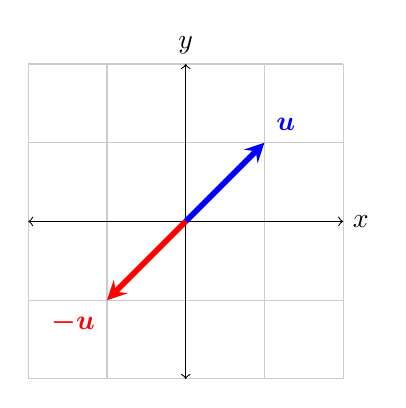
\begin{tikzpicture}
  \draw[thin,gray!40] (-2,-2) grid (2,2);
  \draw[<->] (-2,0)--(2,0) node[right]{$x$};
  \draw[<->] (0,-2)--(0,2) node[above]{$y$};
  \draw[line width=2pt,blue,-stealth](0,0)--(1,1)
        node[anchor=south west]{$\boldsymbol{u}$};
  \draw[line width=2pt,red,-stealth](0,0)--(-1,-1)
        node[anchor=north east]{$\boldsymbol{-u}$};
\end{tikzpicture}
\end{center}
\caption{\label{fig:vectors} Text size inside figure should be as big as
  caption's text.}
\end{figure}
%% %---------------------------


Here's a typical reference to a floating figure:
Figure~\ref{fig:vectors}. Floats should usually be placed where latex
wants then. Figure\ref{fig:vectors} is centered, and has a caption
that instructs you to make sure that the size of the text within the
figures that you use is as big as (or bigger than) the size of the
text in the caption of the figures. Please do. Really.

In our case, we've explicitly drawn the figure inlined in latex, to
allow this tex file to cleanly compile. But usually, your figures will
reside in some file.pdf, and you'd include them in your document
with, say, \textbackslash{}includegraphics.

Lists are sometimes quite handy. If you want to itemize things, feel
free:

\begin{description}
  
\item[fread] a function that reads from a \texttt{stream} into the
  array \texttt{ptr} at most \texttt{nobj} objects of size
  \texttt{size}, returning returns the number of objects read.

\item[Fred] a person's name, e.g., there once was a dude named Fred
  who separated usenix.sty from this file to allow for easy
  inclusion.
\end{description}

\noindent
The noindent at the start of this paragraph in its tex version makes
it clear that it's a continuation of the preceding paragraph, as
opposed to a new paragraph in its own right.


\section{Implementation}
\label{sec:implementation}

We implemented \mdl within the EPaxos framework by modifying the existing implementation of \mpaxos. Our prototype implements a key-value store and consists of 2800 lines of Golang code, not including the testing framework. Our code and experimental scripts are available online ~\cite{code22}. 
% Should the LoC be total or the number of added LOC to existing multi-paxos?


Since \sdl is composable, the unmodified \mpaxos clients submit requests to the leader of a single shard. We extend the clients to issue requests to multiple shard leaders. Clients keep track of a per-shard sequence number, and when requests are concurrent, they include a nonempty dependency set consisting of the previously submitted outstanding requests.
\section{Evaluation}
\label{sec:eval}

% These top level graphs are based on raw data and pick some select points.
% If you want to see the full tput-latency graphs, uncomment the section of graphs at the bottom

%%%%%%%%%%%%%%%%%%%%%%%%%%%%%%%%%%%%%%%%
%%%%%%%%%%%% Uniform fanout %%%%%%%%%%%%
%%%%%%%%%%%%%%%%%%%%%%%%%%%%%%%%%%%%%%%%
\begin{comment}
% Single shard p99 + p50
\begin{figure*}[!htb]
\centering
\subfloat[1 shard p99]{
  \includegraphics[scale=.6]{figs/1shardp99.png}
  \label{fig:1shardp99}
}
\subfloat[1 shard p50]{
  \includegraphics[scale=.6]{figs/1shardp50.png}
  \label{fig:1shardp50}
}
\hspace{0mm}
% 3 shards p99 + p50
\centering
\subfloat[3 shard p99]{
  \includegraphics[scale=.6]{figs/3shardp99.png}
  \label{fig:3shardp99}
}
\subfloat[3 shard p50]{
  \includegraphics[scale=.6]{figs/3shardp50.png}
  \label{fig:3shardp50}
}
\hspace{0mm}
% 9 shards p99 + p50
\centering
\subfloat[9 shard p99]{
  \includegraphics[scale=.6]{figs/9shardp99.png}
  \label{fig:9shardp99}
}
\subfloat[9 shard p50]{
  \includegraphics[scale=.6]{figs/9shardp50.png}
  \label{fig:9shardp50}
}
\caption{p99 and p50 for various shard settings.}
\end{figure*}
\end{comment}

We evaluate \sys{}'s performance handling requests from multi-dispatch clients
compared to Multi-Paxos's performance handling requests from single-dispatch
clients.  We focus on measuring the latency of end-to-end
application-level requests that fan out to multiple data store operations.
%We report on both the p99 and p50 for application-request latency.
%We find p50 a useful metric to look at since our decision to evaluate application-level requests is already end-user facing.
This evaluation aims to answer the following questions:
\begin{enumerate}[leftmargin=*]
    \item How does the end-to-end application latency for \sys{} compare to Multi-Paxos in a datacenter setting?
    \item How does it compare in a wide-area setting?
    \item How does it compare for the Retwis?
    \item How does the throughput of \sys{} compare to Multi-Paxos?
    %, and how is that affected by batching?
    % \item How sensitive is the performance to skewed workloads?
    % \item \todo{Don't work on this yet, we'll almost certainly have to cut it for space.} What is the effect of the first-operation optimization on latency and throughput in a single-shard setting?
\end{enumerate}

% \stale{We show \sys{} has lower throughput than Multi-Paxos for any particular
% number of shards but reduces end-to-end latency for application-level requests
% by up to 75\% when fanout increases and scales with the number of shards. Moreover, we show that \sys{} significantly outperforms Multi-Paxos in a variety of wide-area configurations.}

\subsection{Experimental Setup}
All experiments ran on Cloudlab's Utah platform, using
m510 machines~\cite{duplyakin2019cloudlab}.  Each machine has 1 Intel Xeon-D processor with 8 physical cores
running at 2 GHz (hyper-threading enabled), 64 GB of DDR4-2133 RAM, and a 10
Gb/s NIC\@.  Our setup consists of a 9-node server cluster and 10 additional client machines.
The round-trip latency between all machines is 100--200 $\mu$s.  Each shard has three replicas,
on different physical machines. For multi-sharded single datacenter experiments, we place 9 shards across 3 separate physical machines, ie per machine there are 3 separate shard leader processes, 3 separate replica 1 processes, and 3 separate replica 2 processes. For multi-sharded WAN experiments we place shard leaders on separate physical machines and all replicas are also placed on their own machine, ie per machine there is 1 process. Clients are distributed
evenly across the client machines.

\wl{@anja delete this after reading: the use of texttt I find to be distracting. and when it's printed out by some readers (like me at home) it looks terrible interspersed with regular text so I'm eliminating it.}

% We do not consider failures in this evaluation. Failures degrade performance for
% most protocols but are rare. Thus, \emph{performance} under failures is not a goal
% for either \mpaxos{} or \system{}. Section~\ref{sec:design} describes how \system{}
% handles failures.
% \wl{We can probably cut the preceding paragraph, and if we keep it this is not the right place for it. We should instead talk about it abbove in 7.0 where we talk about we do evaluate too.}


% \al{combine experimental set-up and client design. get rid of metrics, workload,
% failures and replace with, approximately, one sentence each in the experimental
% setup or eval intro}

%\subsection{Client Design}
Clients submit application-level requests. Each application-level request
submits $n$ (the fanout parameter for an experiment) system-level operations. We inject a random delay within a range of 100\,ms before each client issues an application-level request.

Single-dispatch clients interacting with \mpaxos{} have one in-flight operation at
a time. Multi-dispatch clients interacting with \system{} send $n$ system-level
operations concurrently, in order, waiting until all operations complete before
issuing the next batch. Both are closed-loop clients that submit a single
application-level request at a time.
In each experiment, we scale the number of clients issuing requests to both
systems to explore points of low load up through saturation. Our figures report values under low load, around 30\% throughput.
%, including from 2 to 8192 clients.by.

% \al{idk... is it worth noting? If so, not here}
% It's worth noting that since multi-dispatch clients have $n$ requests in-flight at a time, while single-dispatch clients only have 1 request in-flight at a time, \system leaders have to deal with $n$ more requests than \mpaxos at any given time for the same number of clients.

%For a fair comparison between MDL and SDL, we keep the number of outstanding requests sent to each system the same. To achieve this, MDL uses a smaller number of clients $K$ with the specified number $N$ of outstanding requests per client, while SDL uses $K*N$ clients each with 1 outstanding request per client.

% \wl{How does keeping the overall number of requests the same mean the load is the same? We discussed this, you can explain this clearly: keep number of outstanding requests the same in both systems, for mdl this uses a smaller number of clients with the specified number of outstanding requests per client, for sdl its N clients with 1 outstanding request per client.}

%\subsection{Workload}
%We consider uniform and skewed key distributions to explore a more representative range of realistic workloads. For the latter, we generate keys according to a Zipfian distribution with varying skew values $\theta \in \{0.5, 0.7, 0.9, 1.1, 1.3\}$, and use a keyspace of size 1 million.
%
%We do not vary the request type at all, all workloads are 100\% writes, since neither our protocol nor basic Paxos implement op-type specific optimizations.


\subsection{Latency in a Single Datacenter}
\label{sec:shards}
%%%%%%%%%%%%%%%%%%%%%%%%%%%%%%%%%%%%%%%%%%%%%%%%%%%%%%%%%%%%%%%%%%%%%%%%%%%%%%%%%%%
%%%%%%%%%%%%%%%%%%%%%%%%%%%%%%%%%%%%%%%%%%%%%%%%%%%%%%%%%%%%%%%%%%%%%%%%%%%%%%%%%%%
%%%%%%%%%%%%%%%%%%%%%%%%%%%%%%%%%%%%%%%%
%%%%%%%% 1 shard uniform p99 %%%%%%%%%%%
%%%%%%%%%%%%%%%%%%%%%%%%%%%%%%%%%%%%%%%%

% \begin{figure}[!htbp]
% \centering
% \begin{subfigure}[b]{0.9\columnwidth}
% \includegraphics[width=\linewidth]{figs/multicore/interspersed_latencies_multicore.png}
% \caption{First}
% \label{subfig:absoluteMC}
% \end{subfigure}\qquad
% \begin{subfigure}[b]{0.9\columnwidth}
%   \includegraphics[width=\linewidth]{figs/multicore/relative_latencies_multicore.png}
%   \caption{Second}
%   \label{subfig:relateiveMC}
% \end{subfigure}
% \caption{Absolute and normalized p50 latency in a single datacenter setting with 9 shards distributed evenly across a single replication group with 3 replicas. Fanouts of 1--32. Latency for each setting is normalized to the \mpaxos{} latency.}
% \label{fig:DC}
% \end{figure}

\begin{figure}[tbp]
\centering
  \includegraphics[width=.9\linewidth]{figs/multicore/relative_latencies_multicore.png}
\caption{Normalized p50 latency in a single datacenter setting with 9 shards distributed evenly across 3 replicas. Latency for each setting is normalized to the \mpaxos{} latency.}
%p99 latency for a single datacenter setting. We show results for a sweep of fanouts on 1 shard, 3 shards, and 9 shard clusters.}
\label{fig:DC}
\end{figure}
%%%%%%%%%%%%%%%%%%%%%%%%%%%%%%%%%%%%%%%%%%%%%%%%%%%%%%%%%%%%%%%%%%%%%%%%%%%%%%%%%%%
%%%%%%%%%%%%%%%%%%%%%%%%%%%%%%%%%%%%%%%%%%%%%%%%%%%%%%%%%%%%%%%%%%%%%%%%%%%%%%%%%%%

Figure~\ref{fig:DC} compares the median
end-to-end application request latency for \system{} and \mpaxos{}
configured in a single datacenter with a uniform key distribution and fanouts from $1$ to $128$. We show latencies a 9-shard setting.

Recall from \Cref{sec:design} that the latency for \system{} should scale with the fanout as $6T + (N-1)*T$. At a fanout of 1, the latency of application-level requests is roughly the same between \system{} and \mpaxos{}, since the first request in a set of concurrent requests issued to \system{} only requires a single round. Similarly, at a fanout of 2, the latencies are also similar due to the 2-round nature of the protocol for fanouts higher than 1. We expect to see significant latency improvements as the fanout increases past 4, approaching an upper bound of 1/4 as discussed in \Cref{sec:design}.

% In the single shard setting, we do not reach the upper bound due to inefficiencies in our implementation, which is not optimized for the single shard case.
% In a single shard setting, the upper bound cannot be reached due to several reasons. In particular, when the leader is under high load at higher
% fanouts, it must process a large log of buffered
% requests and each of their coordination messages. The protocol evaluated is not optimized for a single shard, so coordination messages are still issued even though the recipient and sender is the same. Lower latency is attenuated by the processing of coordination overhead
% for each request. While not shown, this improvement is even
% greater for p90 and p50, where the tail variability of subrequest latency is less pronounced.
%
%Somewhat counter-intuitively, three shards outperforms nine. 
At 9 shards, we notice latency approaches the lower bound improvement
described in \cref{sec:design} for fanouts $16$ - $128$, with latency
close to 25\% of \mpaxos{}. p90 and p99 latency also approaches 1/4 of \mpaxos{} (not shown).
% An application-level request of fanout $n$ induces
% $n-1$ 1-way inter-shard coordination messages that must be serialized with
% predecessor fault-tolerance and coordination. On the other hand, load balancing
% of large number of requests across multiple shards helps speed the processing
% time at each leader.
%
Overall, \sys{} provides the same latency as \mpaxos{} when there is no potential for parallelization and lower latency when there is potential parallelization at fanouts of 4 or more.

% * Compare e2e app latency in a single datacenter setting\\
% * The latency between clients and shard leader, shard leaders and shard leaders,  and shard leaders and replicas is uniform and low\\

% * Main graph:\\
% * y-axis: latency (yrange starts from 0!)\\
% * x-axis: setting (fanout 1, 2, 8 (or 10), 32)\\
% * bars: show box-and-whiskers plot with (something like) p1, p10, p50, p90, p99 for ellis, and also multi-paxos\\
% * these results should be under relatively moderate load, i.e., choose the highest throughput where both systems still have pretty flat latency (so we aren't see throughput/queuing effects)\\
% * (This looks like the COPS graph I sent you on slack)\\

% * Interpret results \ main takeaway\\
% * fanout 1 is the same because of the optimization\\
% * fanout 2 we have a little bit lower latency, explain\\
% * fanout 10, 32 we have much lower latency, explain\\

% * overall conclusion:\\
% * latency is always the same when there is no potential parallelization (fanout 1) or lower when there is potential parallelization (fanout 2 or more)\\
% * as fanout increases the latency win approachs 3/4\\


\begin{table}[b]
\begin{tabular}{@{}lrrr@{}}
%& \multicolumn{3}{c}{Latencies}  \\
& C $\leftrightarrow$ SL & SL $\leftrightarrow$ SL & SL $\leftrightarrow$ R  \\
Edge Client  & 90\,ms  & 2\,ms & 90\,ms  \\
%Colocated Shards/Clients & 2\,ms  & 2\,ms & 90\,ms  \\
Datacenter Clients    & 2\,ms & 90\,ms & 90\,ms 
\end{tabular}
\vspace{4pt}
\caption{Latencies between Clients \textit{C}, Shard Leaders \textit{SL}, and Replicas \textit{R} for each of the wide-area configurations investigated.}
\label{table:wan}
\end{table}

\subsection{Latency in the Wide Area}
% * Compare e2e app latency in a wide-area setting\\
% * The latency between clients and shard leader, shard leaders to shard leaders, and shard leaders and replicas is heterogenous and can be high depending on the setting\\
% ** we have 3 settings:\\
% ** ...

% * Main graph (one for each setting):\\
% * y-axis: latency (yrange starts from 0!\\
% * x-axis: setting (fanout 1, 2, 8 (or 10), 32)\\
% * bars: show box-and-whiskers plot with (something like) p1, p10, p50, p90, p99 for ellis, and also multi-paxos\\
% * these results should be under relatively moderate load, i.e., choose the highest throughput where both systems still have pretty flat latency (so we aren't see throughput/queuing effects)\\
% * (This looks like the COPS graph I sent you on slack)\\

% * Interpret results \ main takeaway\\
% * do for each setting in turn\\

% * overall conclusion:\\
% * ... \stale{latency is always the same when there is no potential parallelization (fanout 1) or lower when there is potential parallelization (fanout 2 or more)}\\
% * as fanout increases the latency win approaches (shard\_leader -> shard\_leader)/(client->shar\_leader->replica->shard\_leader->client)\\

%We show the results from running \sys{} in the wide area compared with Multi-Paxos in the wide area.
We compare \sys{} to \mpaxos{} for two wide-area configurations with three shards.
%, representative of real world topologies, that show the limits and benefits of using multi-dispatch over Multi-Paxos.
\Cref{table:wan} shows the specifics of the topologies for each of the 2 configurations. We select a wide-area delay of 90\,ms between datacenters and an intra-datacenter latency of 2\,ms. Both of these values are representative of real-world values and provide enough contrast to highlight differences in performance~\cite{wanpings}.

Overall, \Cref{fig:wan} shows that \sys{} is a good choice for the wide-area, since it can parallelize large latencies present in various toplogies. 




\paragraph{Edge Client.}
In this configuration, clients are far from shard leaders to represent when application-level requests are issued from applications running on client edge devices, which is representative of how many applications run today. In addition, we colocate shard leaders which significantly reduces the coordination overhead present in \sys{}.

As seen in \cref{fig:wan}, single-dispatch suffers from having to sequentially pay for the large latency between edge clients and the backend. Moreover, with minimal coordination overhead for \sys{}, the latency of multi-dispatch exceeds the 1/4 limit that exists when latencies are homogeneous.
% \begin{figure*}[tbp]
% \centering
% \subfloat[fanout\xspace1]{
%   \includegraphics[scale=.17]{figs/wan/wide1/wide1-f1.png}
%   \label{fig:w1f1}
% }
% \subfloat[fanout\xspace2]{
%   \includegraphics[scale=.17]{figs/wan/wide1/wide1-f2.png}
% }
% \subfloat[fanout\xspace10]{
%   \includegraphics[scale=.17]{figs/wan/wide1/wide1-f10.png}
% }
% \subfloat[fanout\xspace32]{
%   \includegraphics[scale=.17]{figs/wan/wide1/wide1-f32.png}
% }
% \caption{Edge Client WAN results}

% \label{fig:wan1}
% \end{figure*}
\begin{figure}[tbp]
\centering
  \includegraphics[width=.9\columnwidth]{figs/wan/wide_area_latencies.png}
\caption{Normalized p50 latency in the two wide-area settings with three shards for fanouts of 1--32. Latency for each setting is normalized to the \mpaxos{} latency.}
\label{fig:wan}
\end{figure}

% \paragraph{Colocated Shards and Clients.}
% \todo{Probably going to cut this ... doesn't show much new.}
% In this configuration, clients are in the datacenter and shard leaders remain colocated, to represent geo-replicated settings that benefit from having nearby clients.
% As shown in \Cref{fig:wan}, he perfomrances of the two baselines are similar. Since clients are colocated with shard leaders, single-issue is not the most expensive overhead compared to replication. Moreover, since \sys{} has to pay for two replication rounds between leaders and far away replicas, at high fanouts most of the performance wins are lost.


% \begin{figure*}[tbp]
% \centering
% \subfloat[fanout\xspace1]{
%   \includegraphics[scale=.18]{figs/wan/wide2/wide2-f1.png}
%   \label{fig:w2f1}
% }
% \subfloat[fanout\xspace2]{
%   \includegraphics[scale=.18]{figs/wan/wide2/wide2-f2.png}
% }
% \subfloat[fanout\xspace10]{
%   \includegraphics[scale=.18]{figs/wan/wide2/wide2-f10.png}
% }
% \subfloat[fanout\xspace32]{
%   \includegraphics[scale=.18]{figs/wan/wide2/wide2-f32.png}
% }
% \caption{Colocated Shards+Clients WAN results}
% \label{fig:wan2}
% \end{figure*}

\paragraph{Datacenter Clients and Geo-distributed Clusters.}
In this configuration, we inspect the end-to-end performance of clients located in the datacenter, which is realistic for infrastructure applications that would benefit from the usage of multi-dispatch. Moreover, the shard leaders are not colocated, they are also geo-distributed representing the worst case coordination overhead for \sys{}. We show this configuration to display the limitations of \sys{}, making it the setting for which the benefits of \sys{} are least pronounced. As shown in \Cref{fig:wan}, the limit to \sys{}'s improvement here is closer to $1/2$ the latency of \mpaxos{}. This is because as fanout increases the latency of \sys{} grows with the shard-leader-to-shard-leader latency over 45\,ms, while the latency of \mpaxos{} grows with shard-leader-to-replica-and-back latency of 90\,ms.

% A real world example of this topology might be something like an application that shards disjoint data between two far away geographic regions, and places clients directly between these regions. Within this topology, the coordination between shards is expensive, but issuing requests from clients to each shard is less expensive. In practice, the difference in these 2 latencies will never be as extreme as that depicted here, at best a client can be equidistant from all shards to maintain a consistently low wide-area latency roundtrip. Because of this, we expect \sys{} to still be a better choice for these configurations in the real world.

% \begin{figure*}[tbp]
% \centering
% \subfloat[fanout\xspace1]{
%   \includegraphics[scale=.18]{figs/wan/wide5/wide5-f1.png}
%   \label{fig:w5f1}
% }
% \subfloat[fanout\xspace2]{
%   \includegraphics[scale=.18]{figs/wan/wide5/wide5-f2.png}
% }
% \subfloat[fanout\xspace10]{
%   \includegraphics[scale=.18]{figs/wan/wide5/wide5-f10.png}
% }
% \subfloat[fanout\xspace32]{
%   \includegraphics[scale=.18]{figs/wan/wide5/wide5-f32.png}
% }
% \caption{Datacenter Clients WAN results}
% \label{fig:wan5}
% \end{figure*}

% \subsection{Batching}
% We show evaluation for running \sys{} with batching enabled and compare it to Multi-Paxos with batching enabled. We implement batching using timed batching intervals that range from [250us, 500us, 750us, 1ms, 1.5ms, 2ms, 2.5ms, 3ms, 4ms, 5ms, 10ms]. For Multi-Paxos, client requests are collected for the duration of the batching interval, then all of the prepared requests are replicated together. For \sys{}, we apply this usage of batching for both rounds of the protocol, the initial replication round as well as the secondary ordering round, and use the same batching interval duration for both uses.

% Figure ~\ref{fig:batching} shows the results.

% \begin{figure*}[tbp]
% \centering
% \subfloat[mdl\xspace fanout\xspace1]{
%   \includegraphics[scale=.2]{figs/batching/mdl_f1.png}
% }
% \subfloat[mp\xspace fanout\xspace1]{
%   \includegraphics[scale=.2]{figs/batching/mp_f1.png}
% }
% \subfloat[mdl\xspace fanout\xspace10]{
%   \includegraphics[scale=.2]{figs/batching/mdl_f10.png}
% }

% \subfloat[mp\xspace fanout\xspace10]{
%   \includegraphics[scale=.2]{figs/batching/mp_f10.png}
% }
% \subfloat[mdl\xspace fanout\xspace100]{
%   \includegraphics[scale=.2]{figs/batching/mdl_f100.png}
% }
% \caption{Batching Experiments}
% \label{fig:batching}
% \end{figure*}

\subsection{Retwis}
Retwis is a micro-blogging application~\cite{retwis} for Redis~\cite{redis}, a linearizable key-value store. Retwis has various application-level requests that issue reads and writes to Redis, including user authentication and registration, following and unfollowing, posting messages, and viewing user-specific timelines. We ported Retwis to \mpaxos{} and transform each function, as per Section~\ref{sec:mdl:transform}, to run with \sys{}. We evaluate the impact of \mdl{} on such an application with a synthetic workload (maximum fanout given in ()):
1\% register user (5),
2\% login (3),
2\% logout (3),
10\% post (\# followers),
15\% show profile (2$\times$\# posts),
20\% follow/unfollow (2), and
50\% show timeline (2$\times$\# posts).
%detailed in Table ~\ref{table:retwis}.

Figure~\ref{fig:retwis} shows the median latency for a synthetic workload based on the Retwis application within a single datacenter, using the same 9 shard configuration as shown previously. \sys{} has approximately $1/3$ the latency of \mpaxos{} for the full mixed workload. Some of Retwis's application-level requests are able to take advantage of \Mdl{} better than others. Showing a user's timeline, in particular, approaches \Mdl{}'s theoretical maximum performance. It has a large fanout, as most datastore operations, including getting posts for each user, do not depend on each other. In contrast, functionality such as logging in and out does not provide large improvements, as its sub-operations are mostly data-dependent on each other.

% \begin{table}[h]
% \centering
% \scalebox{0.9}{
%     \begin{tabular}{|c c c|}
%      \hline
%      Application Request Type & \# maximum fanout & workload \% \\ [0.4ex] 
%      \hline
%       Login & 3 & 2\% \\
%       Logout & 3 & 2\% \\
%       Register User & 5 & 1\% \\
%       Post &  $\textit{\# followers}$ & 10\% \\
%       Follow/Unfollow & 2 & 20\% \\
%       Show Timeline  &  $2 \times \textit{\# posts}$  & 50\% \\
%      Show Profile & $2 \times \textit{\# posts}$ & 15\% \\ [1ex] 
%      \hline
%     \end{tabular}
% }
% \caption{Application Request profile for Retwis workload.}
% \label{table:retwis}
% \end{table}

\begin{figure}[tbp]
\centering
  \includegraphics[width=.9\linewidth]{figs/retwis/relative_latencies_retwis.png}
\caption{Retwis p50 latency in a single datacenter  with 9 shards distributed evenly across 3 replicas, normalized to \mpaxos{}.}
%p99 latency for a single datacenter setting. We show results for a sweep of fanouts on 1 shard, 3 shards, and 9 shard clusters.}
\label{fig:retwis}
\end{figure}

% \begin{figure}[!htbp]
% \centering
% \begin{subfigure}[b]{0.9\columnwidth}
% \includegraphics[width=\linewidth]{figs/retwis/interspersed_latencies_retwis.png}
% \caption{First}
% \label{subfig:absolute}
% \end{subfigure}\qquad
% \begin{subfigure}[b]{0.9\columnwidth}
%   \includegraphics[width=\linewidth]{figs/retwis/relative_latencies_retwis.png}
%   \caption{Second}
%   \label{subfig:relateive}
% \end{subfigure}
% \caption{Retwis P50 Latencies in a single datacenter with 9 shards. ~\ref{subfig:absolute} shows the absolute latencies for each of the Retwis functions, while ~\ref{subfig:relateive} shows the latency normalized to \mpaxos{}.}
% \label{fig:retwis}
% \end{figure}

% \subsection{Skew}
% Due to space limitations we omit an experimental comparison of \sys{} and \mpaxos{} for varying values of skew. At a high-level we saw that the improvements of \sys{} over \mpaxos{} are robust to varying skew values until we reached a Zipfian value of above 1.1 where overload at a single shard as a result of the extreme skew degrades the improvement.


\subsection{Throughput}
\label{subsec:eval-tput}
 \cref{fig:tput} in \cref{sec:tput} shows the throughput for fanout 16 using 10 client machines issuing requests to the 9 shard cluster across 3 physical machines. 


\sys{} has about half the max throughput of \mpaxos{}. This is due to the two-round nature of the protocol and the processing of coordination requests at the leader. We also ran experiments with power of 2 fanouts from 1--128 (not shown). Max throughput is nearly identical for fanout 1, similar for fanout 2, and then progressively moves towards 50\% as we get closer to the shown fanout 16 graph. Larger fanouts are similar to fanout 16, with 50\% max throughput.

This is the primary tradeoff of \sys{}: it provides much lower latency than \mpaxos{} but its lower throughput per machine requires more machines to support a given throughput.


% %%%%%%%%%%%%%%%%%%%%%%%%%%%%%%%%%%%%%%%%
% %%%%%%%%%%%% 3 shard skew %%%%%%%%%%%%%%
% %%%%%%%%%%%%%%%%%%%%%%%%%%%%%%%%%%%%%%%%
% \begin{figure*}[tbp]
% \centering
% \subfloat[skew\xspace0.5]{
%   \includegraphics[scale=.2]{figs/3shards_fanout100_skew0.5_8client_CDF.png}
%   \label{fig:3shardsskew}
% }
% \subfloat[skew\xspace0.9]{
%   \includegraphics[scale=.2]{figs/3shards_fanout100_skew0.9_8client_CDF.png}
% }
% \subfloat[skew\xspace1.3]{
%   \includegraphics[scale=.2]{figs/3shards_fanout100_skew1.3_8client_CDF.png}
%   \label{fig:3shardsskewlast}
% }
% \caption{3 shard skew.}
% \end{figure*}


%%%%%%%%%%%%%%%%%%%%%%%%%%%%%%%%%%%%%%%%
%%%%%%%%%%%% 9 shard skew %%%%%%%%%%%%%%
%%%%%%%%%%%%%%%%%%%%%%%%%%%%%%%%%%%%%%%%
% \begin{figure*}[tbp]
% \centering
% \subfloat[skew\xspace0.5]{
%   \includegraphics[scale=.2]{figs/old/9shards_fanout100_skew0.5_8client_CDF.png}
%   \label{fig:9shardsskew}
% }
% \subfloat[skew\xspace0.9]{
%   \includegraphics[scale=.2]{figs/old/9shards_fanout100_skew0.9_8client_CDF.png}
% }
% \subfloat[skew\xspace1.3]{
%   \includegraphics[scale=.2]{figs/old/9shards_fanout100_skew1.3_8client_CDF.png}
%   \label{fig:9shardsskewlast}
% }
% \caption{9 shard skew.}
% \end{figure*}

% %%%%%%%%%%%%%%%%%%%%%%%%%%%%%%%%%%%%%%%%%%%%%%%%%%%%%%%%%%%%%%%%%%%%%%%%%%%%%%%%%%%
% %%%%%%%%%%%%%%%%%%%%%%%%%%%%%%%%%%%%%%%%%%%%%%%%%%%%%%%%%%%%%%%%%%%%%%%%%%%%%%%%%%%
% %%%%%%%%%%%%%%%%%%%%%%%%%%%%%%%%%%%%%%%%%%%%%%%%%%%%%%%%%%%%%%%%%%%%%%%%%%%%%%%%%%%

% % \Crefrange{fig:3shardsskew}{fig:3shardsskewlast} and
% % ~\ref{fig:9shardsskew}--\ref{fig:9shardsskewlast} show various skew values for
% % the 3-shard and 9-shard configurations. 

% \Crefrange{fig:9shardsskew}{fig:9shardsskewlast} and
% show various skew values for
% the 9-shard configurations. 
% (Figures for a 3-shard configuration are similar and are omitted due to space constraints.)


% We generate keys according to a Zipfian
% distribution with varying skew values $\theta \in \{0.5, 0.9, 1.3\}$,
% and use a keyspace of size 1 million. We look at CDFs for application-level
% requests with fanout 100 issued by 8 concurrent clients.

% Increasingly higher skew approaches single shard performance, where \system's
% coordination is cheaper, as it does not include network latency, but experiences
% overload sooner.  Overall skew has little impact on end-to-end latency until a
% high skew value of 1.3, where the tail latency for application-level requests
% starts increasing at lower percentiles, by about 2x. We notice this degradation
% begin earlier at around skew 1.1 as well. We expect much of this is due to the
% high load on the leader responsible for highly contentious keys.

% \subsection{Single-Shard Optimization}
% We investigate the performance of a modification to the multi-dispatch protocol optimized for the single-shard setting, and compare it with the original multi-dispatch protocol as well as multi-paxos. The main modifications include removing coordination messages and removing the 2nd “ordering” round between leaders and replicas for all requests, as the first and only round replicates both a request as well as its index in the log. We keep the sequence numbers and buffer requests that arrive out-of-order wrt to their expected next sequence number.
% \begin{figure*}[tbp]
% \centering
% \subfloat[Fanout\xspace1]{
%   \includegraphics[scale=.2]{figs/ssa/ssa_f1.png}
%   \label{fig:SSA_f1}
% }
% \subfloat[Fanout\xspace10]{
%   \includegraphics[scale=.2]{figs/ssa/ssa_f10.png}
%   \label{fig:SSA_f2}
% }
% \subfloat[Fanout\xspace100]{
%   \includegraphics[scale=.2]{figs/ssa/ssa_f100.png}
%   \label{fig:SSA_f10}
% }
% \caption{Single-Shard Optimizations for fanouts 1, 10, 100}
% \label{fig:SSA}
% \end{figure*}

% As shown in figure ~\ref{fig:SSA}, without the optimizations, MDL cannot offer the same performance as SDL in the single-shard setting due to the overhead of coordination requests. With the optimizations, however, MDL can provide significantly higher throughput and lower latencies than SDL.

\begin{comment}
\subsection{MDL with Geo-rep in the Wide Area}
\label{sec:wide}
We show the e2e app. latency for varying inter-shard latency (which we call the wide area **this might be wrong terminology) and inter-replica latency (which we call geo-replication, also might be wrong terminology).

\subsection{Applications on MDL}
\label{sec:apps}

As described in prior sections, we built a tool to automatically transform applications built to interact with SDL backends to interact with MDL backends, maintaining external equivalence. In this section we select 3 representative applications, A1, A2, A3, and show that when transformed with our tool, all 3 see an improvement in e2e latency. We use DeathStar to benchmark the applications.

A1 is an application that ....

A2 is an application that ...

A3 is an application that ...

We expect transformed applications that have a large degree of data parallelism and are read heavy running on MDL backends to see the largest e2e latency improvements over their pre-transformed counterparts running on SDL backends.

Jeff is still looking for these applications at the moment -- it would be good to pick applications that are read heavy and some that are mixed. All should include varying degrees of data parallelism, to show how some improve after the transformation more than others.
\end{comment}


\section{Related Work}
\label{sec:related}

\wl{Should discuss this paper: https://www.dpss.inesc-id.pt/~rodrigo/antipode-sosp2023.pdf}

\paragraph{Consistency Models.}
The core difference between Linearizability and \mdl{} is that \mdl{} enforces issue-ordering for operations from the same application process, even concurrent ones.
Using issue ordering as the constraint is intuitive and thus conceptually matches earlier work.
Session guarantees~\cite{terry1994session} introduces four guarantees for operations within a given session: read-your-writes, monotonic reads, writes-follow-reads, and monotonic writes. When a session corresponds to an application process handling a user request the combination of these four guarantees ensures issue ordering.
Similarly, A-Linearizability~\cite{hunt2010zookeeper} requires an issue-order for multi-dispatched writes. 

This earlier work, however, does not provide `strong' consistency comparable to Linearizability.
Session guarantees do not ensure any real-time order, e.g., a write that finished yesterday might not been seen by a read issued today.
A-Linearizability, despite its name, only provides Linearizability-like consistency for write operations but also has stale reads.
Thus, \Mdl{} is distinct from this earlier work it builds on by providing `strong' Linearizability-like consistency for all operations.

Sequential consistency was originally described in the context of
multi-processors~\cite{lamport1979sequential}. It requires that
the system reflects a total order over all operations that is 
consistent with each processor's `program order.' It is often
interpreted as allowing processors to issue multiple memory 
operations concurrently, as is common in computer architecture.
But in the distributed systems community, it has often
included the assumption that each process issues operations 
sequentially~\cite{attiya1993seqlin}.

But like other, weaker consistency
models~\cite{ahamad1995causal,lloyd2011cops,terry1995bayou,deCandia2007dynamo, antipode}, 
sequential consistency introduces a trade-off. Although it enables
better-performing systems, it makes building correct applications more difficult, especially since applications today interact with many different services that provide unique consistency guarantees. In contrast, through its transformation
and accompanying equivalence result, \MDL{} offers transformed
applications better performance while guaranteeing they behave 
identically to the original application.

\paragraph{Equivalence Results.}
Other works have used the idea of equivalence to various
ends~\cite{goldman1993unifiedModel,lundelius1984clocksync,
fischer1985flp,attiya1993seqlin},
such as proving bounds on clock
synchronization~\cite{lundelius1984clocksync}.
Most similar to our work is Helt et al.~\cite{helt2021rss}, which shows that their consistency
models provided identical correctness guarantees for applications
as strict serializability~\cite{papadimitriou1979serializability} and linearizability~\cite{herlihy1990linearizability}.
They refer to this as ``invariant equivalence.'' 

External equivalence provides a proves a different property.
It does not guarantee that the original and transformed applications
will transition through the same states and thus obey the same
application invariants. Instead, it guarantees that users cannot distinguish between the two
application versions.
Conversely, invariant-equivalent applications may exhibit different
user-facing behaviors (referred to as ``anomalies'' in Helt et
al.~\cite{helt2021rss}), so they are not necessarily externally equivalent.
We leave further investigation into
\MDL{}'s impacts on application invariants to future work.

\paragraph{Linearizable Systems.} Many protocols have been developed to provide fault-tolerant, linearizable storage.
State-of-the-art leader-based
protocols~\cite{ongaro2014raft,lamport1998paxos,oki1988vr},
suffer in wide-area deployments due to the extra
latency incurred between application processes and (potentially far)
leaders.
There is a body of work that improves the performance of
linearizable systems in the wide
area~\cite{mao2008mencius,moraru2013epaxos,burke2020gryff} and that can sometimes avoid the latency penalty from a far-away leader.
As a leader-based protocol \sys{} must pay the penalty for far-away leaders.
An interesting avenue for future work is removing this penalty by adding \mdl{} to some of these designs.

Other systems ~\cite{salus} provide \mdl{}, but with severe restrictions on the concurrency of clients and their programming behavior, while \system{} does not.

\paragraph{Transactional Systems.}
Transactional consistency models, like strict serializability,
allow application processes to group their operations into
transactions~\cite{papadimitriou1979serializability}. Such
systems generally guarantee that the operations in a transaction
will take effect atomically, as one indivisible unit (although weaker 
guarantees also exist~\cite{adya1999weakcons}).
Compared to \MDL{}'s issue order guarantee, transactional atomicity 
is stronger since it prevents other processes from observing 
intermediate states where some of the operations in a transaction 
have taken effect but not others. 

% A closer investigation
% of the relationship between these guarantees (and its
% implications for application correctness) is left to future work.

Some transactional consistency
models~\cite{papadimitriou1979serializability,adya1999weakcons} similarly assume 
each application process issues one transaction at a time. This may 
make it possible to combine the ideas here with that of transactions. 
This may offer similar improvements in end-to-end 
performance for application built atop existing transactional 
systems~\cite{thomson2014calvin,mahmoud2013replicatedCommit,zhang2018tapir,mu2014rococo,mu2016janus,kraska2013mdcc,ren2019slog,taft2020crdb,yan2018carousel}.







\section{Conclusion}
\label{sec:concl}

This work presents a new consistency model, \mdllong{}, a
modern extension of linearizability that explicitly allows
client processes to issue multiple operations concurrently.
We also describe how
to transform applications that currently interact with 
a linearizable system into ones that can reap the performance
benefits offered by a comparable \mdl{} system. We prove that
following the transformation ensure the new application will 
behave the same as the old. Further, we design, implement,
and evaluate \sys{}, the first
multi-shard system to guarantee \mdl{}. Our evaluation 
demonstrates \sys{} offers significant (e.g., up to 75\%) 
reductions in end-to-end application latency.

%-------------------------------------------------------------------------------
\section*{Acknowledgments}
%-------------------------------------------------------------------------------

The USENIX latex style is old and very tired, which is why
there's no \textbackslash{}acks command for you to use when
acknowledging. Sorry.


%-------------------------------------------------------------------------------
\bibliographystyle{ACM-Reference-Format}
\bibliography{paper,venues}

% \clearpage
% \appendix

% \section{External Equivalence Proof}
\label{sec:equivalence}

In this section, we first define some preliminaries and then use them to show
that an application built atop a linearizable service can be transformed to take
advantage of the concurrency offered by \multidispatch{} linearizability such that
the two versions of the application are externally equivalent. Our formalism
closely aligns with that of prior work~\cite{helt2021rss}, which leverages the
formalism of I/O automata~\cite{lynch1987ioa,lynch1996da}.

\subsection{Preliminaries}
\label{sec:equivalence:preliminaries} 

\subsubsection{I/O Automata}
\label{sec:equivalence:preliminaries:ioa}

We model each component in our system as an I/O automaton
(IOA)~\cite{lynch1987ioa,lynch1996da}, a type of state machine. Each
transition of an IOA is labeled with an \textit{action}, which can be an
\textit{input}, \textit{output}, or \textit{internal} action. Input and output
actions allow the automaton to interact with other IOA and the environment. We
assume input actions are not controlled by an IOA---they may arrive at any time.
Conversely, output and internal actions are \textit{locally controlled}---an IOA defines
when they can be performed.

To specify an IOA, we must first specify its \textit{signature}. A signature $S$ is
a tuple comprising three disjoint sets of actions: input actions $\actin(S)$,
output actions $\actout(S)$, and internal actions $\actint(S)$. We also define
$\localacts(S) = \actout(S) \cup \actint(S)$ as the set of locally controlled actions, $\extacts(S) = \actin(S) \cup \actout(S)$ as the set of external actions, and $\acts(S) = \actin(S) \cup \actout(S) \cup \actint(S)$ as the set of all actions.

Formally, an I/O automaton $A$ comprises four items:
\begin{enumerate}
\item a signature $\sig(A)$,
\item a (possibly infinite) set of states $\states(A)$,
\item a set of start states $\start(A) \subseteq \states(A)$, and
\item a transition relation $\trans(A) \subseteq \states(A) \times
  \acts(\sig(A)) \times \states(A)$.
\end{enumerate}
Since inputs may arrive at any time, we assume that for every state $s$ and
input action $\pi$, there is some $(s, \pi, s^\prime) \in \trans(A)$.

An \textit{execution} of an I/O automaton $A$ is a finite or infinite
sequence of alternating states and actions $s_0,\pi_1,s_1,\ldots$ such that for
each $i \geq 0$, $(s_i, \pi_{i+1}, s_{i+1}) \in \trans(A)$ and $s_0 \in \start(A)$. Finite executions always end with a state.

Given an execution $\alpha$, we can also define
its \textit{schedule} $\sched(\alpha)$, which is the subsequence of just
the actions in $\alpha$. Similarly, an execution's \textit{trace}
$\trace(\alpha)$ is the subsequence of just the external actions $\pi \in
\extacts(A)$.

\subsubsection{Composition and Projection}
\label{sec:equivalence:preliminaries:composition}

To compose
two IOA, they must be \textit{compatible}. Formally, a finite set of
signatures $\{S_i\}_{i \in I}$ is compatible if for all $i,j \in I$ such that $i \neq j$:
\begin{enumerate}
\item $\actint(S_i) \cap \acts(S_j) = \emptyset$, and
\item $\actout(S_i) \cap \actout(S_j) = \emptyset$.
\end{enumerate}
A finite set of automata are compatible if their signatures are compatible.

Given a set of compatible signatures, we define their \textit{composition} $S =
\prod_{i \in I} S_i$ as the signature with $\actin(S) = \bigcup_{i \in I}
\actin(S_i) - \bigcup_{i \in I} \actout(S_i)$, $\actout(S) = \bigcup_{i \in I}
\actout(S_i)$, and $\actint(S) = \bigcup_{i \in I} \actint(S_i)$.

The composition of a set of compatible IOA yields the automaton $A =
\prod_{i \in I} A_i$ defined as follows:
\begin{enumerate}
\item $\sig(A) = \prod_{i \in I} \sig(A_i)$,
\item $\states(A) = \prod_{i \in I} \states(A_i)$,
\item $\start(A) = \prod_{i \in I} \start(A_i)$, and
\item $\trans(A)$ contains all $(s,\pi,s^\prime)$ such that for all $i \in I$, if $\pi \in \acts(\sig(A_i))$, then $(s_i,\pi,s_i^\prime) \in \trans(A_i)$ and otherwise, $s_i = s_i^\prime$.
\end{enumerate}
The states of the composite automaton $A$ are vectors of the states of the composed
automata. When an action occurs in
$A$, all of the component automata with that action each take a step simultaneously, as defined
by their individual transition relations. The resulting state differs in each of
the components corresponding to these automata, and the other components are
unchanged. We denote the composition of a small number of
automata using an infix operator, e.g., $A \times B$.

Given the execution $\alpha$ of a composed automaton $A = \prod_{i \in I} A_i$,
we can \textit{project} the execution onto one of the component automata $A_i$.
The execution $\alpha|A_i$ is found by removing all actions from
$\alpha$ that are not actions of $A_i$. The states of $\alpha|A_i$ are
given by the $i$th component of the corresponding state in $\alpha$. The
projection of a trace is defined similarly.

Further, we can write the projection of a state $s$ of $A$ on $A_i$ as $s|A_i$. 
Finally, we can also project $\trace(\alpha)$ onto a set of actions $\Pi$ where
$\trace(\alpha)|\Pi$ yields the subsequence of $\trace(\alpha)$ containing only actions in $\Pi$.

\subsubsection{Channels}
\label{sec:equivalence:preliminaries:channels}

\begin{table}[!t]
  \centering
  \begin{tabular}{l l l}
    \multicolumn{3}{l}{\textbf{Signature:}} \\ \hline
    Inputs: & & Outputs: \\
    $\sendto(m)_{ij}, m \in M$ & & $\sent_{ij}$ \\
    $\recvfrom_{ij}$ & & $\receive(m)_{ij}, m \in M$ \\ \hline
    \\
    \multicolumn{3}{l}{\textbf{States:}} \\ \hline
    \multicolumn{3}{l}{$Q$, a FIFO queue of elements of $M$, initially empty} \\
    \multicolumn{3}{l}{$e$, a Boolean, initially \textit{false}} \\
    \multicolumn{3}{l}{$r$, a Boolean, initially \textit{false}} \\ \hline
    \\
    \multicolumn{3}{l}{\textbf{Actions:}} \\ \hline
    \multicolumn{2}{l|}{$\sendto_{ij}(m)$:} & $\sent_{ij}$: \\
    \multicolumn{2}{l|}{Precondition: \textit{true}} & Precondition: $e$ \\
    \multicolumn{2}{l|}{Effect: $\textsc{Push}(Q,m); e \gets \textit{true}$} & Effect: $e \gets \textit{false}$ \\
    \hline \hline
    $\recvfrom_{ij}$: & \multicolumn{2}{|l}{$\receive_{ij}(m)$:} \\
    Precondition: \textit{true} & \multicolumn{2}{|l}{Precondition: $r \land m = \text{Head}(Q)$} \\
    Effect: $r \gets \textit{true}$ & \multicolumn{2}{|l}{Effect: $\textsc{Pop}(Q); r \gets \textit{false}$} \\ \hline
  \end{tabular}
  \captionof{figure}{Buffered Channel I/O Automaton}
  \label{fig:buffered-channel-ioa}
\end{table}

Each pair of processes in our system communicates via a pair of FIFO
channels that are asynchronous, reliable, and buffered. Each
channel's signature, states, and actions are specified in
Figure~\ref{fig:buffered-channel-ioa}.

We denote the channel that process $i$ uses to send messages to process $j$ as
$C_{ij}$. $C_{ij}$ has two sets of input actions, $\sendto_{ij}(m)$ and
$\recvfrom_{ij}$, and two sets of output actions, $\sent_{ij}$ and
$\receive_{ij}(m)$, for all $m$ in some space of messages $M$. Process $i$ has
corresponding output actions, $\sendto_{ij}(m)$ and $\recvfrom_{ji}$, and input
actions, $\sent_{ij}$ and $\receive_{ji}(m)$, for all other processes $j$ and
messages $m$. To send a message to process $j$, process $i$ takes a
$\sendto_{ij}$ step, and $C_{ij}$ subsequently takes a $\sent_{ij}$ step.
Similarly, to receive a message from $C_{ij}$, process $j$ takes a
$\recvfrom_{ij}$ step, and $C_{ij}$ subsequently takes a $\receive_{ij}(m)$ step.

The modeling of buffering in the channels differs from past
work~\cite{lynch1996da}. There, receive-from actions are omitted, and received
actions are modeled as output actions of channels and corresponding input
actions of processes. This implies processes cannot control when they
change their state in response to a message.

But in real applications, this is unrealistic. Although the network stack of a
machine may accept and process a packet at any time, application code controls
when it processes the contained message. For instance, the packet's contents remain in a kernel buffer until the application performs a read system call
on a network socket. This control is essential to our proof as it ensures
application processes do not receive messages while waiting for responses from
services.

We say an execution $\alpha$ of a channel $C_{ij}$ is \textit{well-formed} if
(1) $\trace(\alpha) | \{\sendto_{ij}(m)\}_{m \in M} \cup \{\sent_{ij}\}$ is a
sequence of alternating send-to and sent actions, starting with a send-to; and
similarly (2) $\trace(\alpha) | \{\recvfrom_{ij}\} \cup \{\receive_{ij}(m)\}_{m
  \in M}$ is a sequence of alternating receive-from and received actions,
starting with a receive-from.

\subsubsection{Types and Services}
\label{sec:equivalence:preliminaries:services}

Processes in our system interact with \textit{services}, each with a specified
\textit{type}~\cite{herlihy1990linearizability,lynch1996da}. A service's type
$\type$ defines its set of possible \textit{values} $\vals(\type)$, an
\textit{initial value} $v_0 \in \vals(\type)$, and the \textit{operations}
$\ops(\type)$ that can be invoked on the service. Each operation $o \in
\ops(\type)$ is defined by a pair of sets of actions: \textit{invocations} $\invs(o)$ and
\textit{responses} $\resps(o)$. Each contains subscripts denoting a unique service name and a process index. An invocation and response \textit{match} if their subscripts are equal.
Finally, each service has a \textit{sequential specification} $\spec$, a
prefix-closed set of sequences of matching invocation-response pairs.

For example, consider a read/write register $x$ that supports a set of $n$
processes and whose values is the set of integers. The read operation would then
be defined with invocations $\{\textsc{read}_{i,x}\}$ and responses
$\{\textsc{ret}_{i,x}(j)\}$ for all $0 \leq i \leq n$ and $j \in \mathcal{N}$.
Similarly, the write operation would have invocations
$\{\textsc{write}_{i,x}(j)\}$ and responses $\{\textsc{ack}_{i,x}\}$. Finally,
its sequential specification would be the set of all sequences of reads and
writes such that reads return the value written by the most recent write or the
initial value if none exists.

\subsubsection{System Model}
\label{sec:equivalence:preliminaries:model}

We model a distributed application as the composition of two finite sets of I/O
automata: processes and channels. $n$ denotes the number of processes, so there are $n^2$ channels. The processes execute the application's code by performing local computation, exchanging messages via channels, and performing invocations on and receiving responses from services.

In the results below, we are interested in reasoning about the processes' external behaviors while assuming various correctness conditions of the services they interact with. Thus, we do not model services as IOA. Instead, we assume the processes interact with a service with an arbitrary type $\type$ and $\spec$ defined for $n$ processes.

For each operation $o \in \ops(\type)$, process $P_i$ is then assumed to have an output action for every invocation action in $\invs(o)$ with process index $i$. Similarly, $P_i$ has an input action for every response action in $\resps(o)$ with process index $i$. We refer to these input and output actions as a process's \textit{system-facing} actions $\system(P_i)$.

To model stop failures, we assume each process $P_i$ has an input
action $\textit{stop}_i$ such that after receiving it, $P_i$ ceases taking
steps. If $\textit{stop}_i$ occurs while $P_i$ is waiting for a response from a service, then we assume the service does not return a response. But the operation may still cause a service's state to change, and this change may be visible to operations by other processes.

Finally, to allow the distributed application to receive input from and return values to its environment (e.g., users), we assume each $P_i$ has a set of \textit{user-facing} actions $\user(P_i)$. Similar to a process's interactions with services, a user's interaction with a process is modeled through input-output pairs of user-facing actions.

We make two final assumptions about the processes: First, we assume that while
each process has access to a local clock, which is part of its state, and may
set local timers, which are internal actions, the process makes no assumptions
about the drift or skew of its clock relative to others. Second, processes only
invoke an operation on a service when they have no outstanding send-to or
receive-from actions at any channels.

Let $P = \prod_{i \in I} P_i$ be the composition of the $n$ processes and
$C = \prod_{1 \leq i \leq n} \prod_{1 \leq j \leq n} C_{ij}$ be the composition of $n^2$ channels.
Let $\alpha$ be an execution of the distributed application $P \times C$.

$\alpha$ is \textit{well-formed} if it satisfies three criteria:
First, for all $P_i$, $\trace(\alpha) | \system(P_i)$ must be a sequence of alternating invocation and matching response actions, starting with an invocation. Second, for all $C_{ij}$, $\alpha | C_{ij}$ is well-formed. Third, for all $P_i$, $P_i$ does not take an output step while waiting for a response from some service. 

\subsubsection{External Equivalence}
\label{sec:equivalence:preliminaries:equivalence}

Two executions, $\alpha$ and $\beta$, are
\textit{externally equivalent} if $\alpha|U = \beta|U$. Intuitively,
externally equivalent executions are indistinguishable to users.

\subsubsection{Transformation}
\label{sec:equivalence:preliminaries:transform}

A single-dispatch application $A$ must be transformed to take advantage of the benefits offered by a multi-dispatch system. We use the notation $A^\prime = \transform(A)$ to denote applying the transformation to each process within $A$, i.e., $A^\prime = \prod_i P^\prime_i = \prod_i \transform(P_i)$.

We define $\transform$ as follows: We first replace all synchronous, system-facing I/O with futures. This allows operation invocations and responses to be reordered in $A$ with respect to other actions (i.e., instructions). The aim is to then move operation invocations earlier such that the application can issue multiple operations concurrently and reap the performance benefits of an MD-Linearizable system.
To produce $A^\prime$, we then move actions in $A$ before prior actions provided $A^\prime$ maintains the following:

    \textbf{(R1)} the order of data-dependent actions within each process of $A$,
    
    \textbf{(R2)} the control flow of each process in $A$,
    
    \textbf{(R3)} the issue order of $A$’s operations,
    
    \textbf{(R4)} the order of non-system-facing external actions in $A$, including messages to/from users and between processes,
    
    \textbf{(R5)} the order between a non-system-facing external actions and operation invocations (in particular, the first invocation in a sequence of operations), and
    
    \textbf{(R6)} the order between non-system-facing external actions and operation responses (e.g., by waiting for the successful responses of any outstanding operations before sending a message to a user).

\subsection{Equivalence Proof}
\label{sec:equivalence:proof}

\begin{thm}
 Let $A^\prime = \transform(A)$. Suppose $\alpha^\prime$ is a finite execution of $A^\prime \times C$ that satisfies multi-dispatch real-time precedence. Then there exists a single-dispatch well-formed, finite execution $\alpha$ of $A \times C$ that satisfies single-dispatch real-time precedence such that $\alpha^\prime | U = \alpha | U$.
\end{thm}

\begin{proof}
  Let $A^\prime$, $A$, and $C$ be defined as above, and let $\alpha^\prime$ be an arbitrary finite execution of $A^\prime \times C$ that satisfies multi-dispatch real-time precedence.

  The proof proceeds in three steps: First, we create an execution $\beta^\prime$ from $\alpha^\prime$ by essentially undoing the parallelizing transformation in each process's sub-execution. Second, we produce $\beta$ from $\beta^\prime$ by removing any incomplete or failed operations. Third, we produce $\alpha$ from $\beta$ by fixing the order of actions across processes to ensure $\alpha$ is well-formed and satisfies real-time precedence.

  By the assumption that $A$ only produces single-dispatch well-formed executions and rules \textbf{R4}, \textbf{R5}, and \textbf{R6} of $\transform$, $\alpha^\prime$ is multi-dispatch well-formed, so each $\alpha^\prime | P_i$ comprises sub-sequences of local and system-facing actions separated by non-system-facing external actions. Further, by \textbf{R4}, the order of the non-system-facing external actions in each $\alpha^\prime | P_i$ respects the program order of the original $A$.

  We first reorder the actions in each sub-sequence of each $\alpha^\prime | P_i$ to place the local and system-facing actions such that they respect $A$'s program order. More precisely, for each $\alpha^\prime | P_i$, starting with the right-most action $\pi_1$, shift $\pi_1$ left in $\alpha^\prime$ until it precedes all other actions $\pi_2$ such that $A$'s program order requires it. Let $\beta^\prime$ be the resulting execution.

  By assumption, $\alpha^\prime$ satisfies multi-dispatch real-time precedence, so let $<_S$ be a total order over the operations in $\alpha^\prime$ (and thus $\beta^\prime$). Observe that by the process above, each $\beta^\prime | P_i$ now issues its operations sequentially (since $A$'s program order requires it). Further, by the definition of multi-dispatch real-time precedence (in particular its suffix-closed failure semantics) all of a process's completed operations precede any incomplete or failed ones. For each $\beta^\prime | P_i$, remove any trailing system-facing actions corresponding to operations that are either failed or not present in $S$ as well as any trailing local actions to ensure it remains a valid process sub-execution. Let $\beta$ be the resulting execution.

  Since the order of the non-system-facing external actions in each $\alpha^\prime | P_i$ already respects the program order of the original $A$, these actions are not reordered by the steps above. Thus, the order of non-system-facing actions in $\beta^\prime | P_i$ and thus $\beta | P_i$ also respects $A$’s program order. 

  But $\beta$ may not satisfy real-time precedence. To remedy this and produce the needed $\alpha$, we next define an order over the actions in $\beta$ that combines the order of each process’s (now single-dispatch) sub-execution in $\beta$ with the total order of operations guaranteed by MDL from the original $\alpha^\prime$. To ensure $\alpha$ is single-dispatch well-formed, the order also preserves the order of send-to and receive-from actions used to transmit messages between processes and users.

  Let $\prec_\beta$ be the transitive closure of the following pairs of actions $(\pi_i, \pi_j)$ in $\beta$:
  \begin{enumerate}
      \item $\mathbf{\prec_{P_i}}$\textbf{:} $\pi_i$ precedes $\pi_j$ in some $\beta | P_i$,
      \item $\mathbf{\prec_S}$\textbf{:} for each adjacent pair of operations $o_k$, $o_{k+1}$ in $S$, $\pi_i$ is the response action of $o_k$ and $\pi_j$ is the invocation action of $o_{k+1}$,
      \item $\mathbf{\prec_M}$\textbf{:} $\pi_i$ is a send action for some message $M$ (from a user to a process, a process to a user, or between two processes) and $\pi_j$ is its corresponding receive action, or
      \item $\mathbf{\prec_U}$\textbf{:} $\pi_i$ precedes $\pi_j$ in $\beta | U$.
  \end{enumerate}

  We posit $\prec_\beta$ defines an irreflexive partial order over the actions in $\beta$. Clearly it is transitive; we now prove it is acyclic and irreflexive.

  For sake of contradiction, assume $\prec_\beta$ contains at least one cycle. Let $\pi_1 \prec_\beta \pi_2 \prec_\beta \ldots \prec_\beta \pi_1$ be a shortest cycle that does not contain any transitive edges.

  We begin by proving an important lemma (Lemma~\ref{lemma:helper2}) regarding sequences of actions connected by $\prec_\beta$. We use this lemma in the remainder of the proof.

  \begin{lem}
    Let $\pi_1 \prec_\beta \ldots \prec_\beta \pi_m$ be a sequence of $m$ actions connected only by $\prec_{P_i}$ and $\prec_S$ edges, and further assume $\pi_1$ and $\pi_m$ are send-to or receive-from actions. Then $\pi_1$ precedes $\pi_m$ in $\beta$.
    \label{lemma:helper1}
  \end{lem}
  \begin{proof}
      We proceed by cases:

      $\mathbf{m=2}$\textbf{.} Since they are send-to or receive-from actions, $\pi_1$ and $\pi_2$ must be connected by a $\prec_{P_i}$ edge, so $\pi_1$ precedes $\pi_2$ by the definition of $\prec_{P_i}$.

      $\mathbf{m=3}$\textbf{.} By similar reasoning, the two edges must be $\prec_{P_i}$ edges for some $P_i$, so $\pi_1$ precedes $\pi_3$ again by the definition of $\prec_{P_i}$.

      $\mathbf{m \geq 4}$\textbf{.} By the same reasoning, the conclusion is true if all of the edges are $\prec_{P_i}$ for some $P_i$, so assume there is at least one $\prec_S$ edge.
      Then the sequence has the following structure:
      $\pi_1 \prec_{P_1} \ldots \prec_{P_1} \pi_i \prec_S \pi_{i+1} \prec_{P_2} … \prec_{P_2} \pi_j \prec_S \pi_{j+1} … \pi_k \prec_S \pi_{k+1} \prec_{P_n} … \prec_{P_n} \pi_m$.

      Note the first and final edges cannot be $\prec_S$ edges because by assumption $\pi_1$ and $\pi_m$ are send-to or receive-from actions.

      By the definition of $\prec_S$, $\pi_i$ is a response action for some operation invoked by $P_1$. By the definition of $\prec_{P_1}$, $\pi_1$ precedes $\pi_i$ in $\beta | P_1$. Since $\alpha^\prime$ is multi-dispatch well-formed and $A$, by assumption, only produces single-dispatch well-formed executions, the reordering above to produce $\beta^\prime$ and thus $\beta$ must have maintained the relative order of $\pi_1$ (a send-to or receive-from action) and any subsequent invocation or response actions at $P_1$. It follows that since $\pi_1$ precedes $\pi_i$ in $\beta | P_1$, it must also precede $\pi_i$’s corresponding invocation $\inv(\pi_i)$ in $\beta | P_1$. Since the relative order of $\pi_1$ and $\inv(\pi_i)$ is the same in $\alpha^\prime$ and $\beta$, this implies $\pi_1$ must also precede $\inv(\pi_i)$ in $\alpha^\prime | P_1$.

      By the definition of $\prec_S$, $\prec_{k+1}$ is an invocation action at $P_n$. By similar reasoning as above, we can conclude that $\pi_{k+1}$’s corresponding response $\resp(\pi_{k+1})$ must precede $\pi_m$ in $\beta | P_n$ and thus $\alpha^\prime | P_n$. Thus, we have $\pi_1$ precedes $\inv(\pi_i)$ and $\resp(\pi_{k+1})$ precedes $\pi_m$ in $\alpha^\prime$.

      Now consider $\pi_{i+1} \prec_{P_2} \ldots \prec_{P_2} \pi_j$. $\pi_{i+1}$ is an invocation, and $\pi_j$ is a response. By the definition of $\prec_{P_2}$, $\pi_{i+1}$ precedes $\pi_j$ in $\beta | P_2$. Further, $P_2$’s system interactions occur sequentially in $\beta$, so $\pi_{i+1}$ must also precede $\pi_j$’s corresponding invocation in $\beta | P_2$. By \textbf{R3}, the transformation between $A$ and $A^\prime$ preserves each process’s invocation order, so this implies $\pi_{i+1}$ must precede $\pi_j$’s corresponding invocation in $\alpha^\prime | P_2$.

      By the definition of MDL, the operations in $S$ respect this invocation order, too, so $\op(\pi_{i+1})$ is ordered in $S$ before $\op(\pi_j)$. We can apply the same reasoning to conclude the same about any similar sub-sequence. For example, we can conclude $\op(\pi_{j+1})$ is ordered in $S$ before $\op(\pi_k)$.

      Combined with $\pi_i \prec_S \pi_{i+1}$, $\pi_j \prec_S \pi_{j+1}$, and so on, we can thus conclude that $\op(\pi_i)$ is ordered in $S$ before $\op(\pi_{k+1})$. Then it must be the case that $\inv(\pi_i)$ precedes $\resp(\pi_{k+1})$ in $\alpha^\prime$ because otherwise, by the real-time guarantees of MDL, $\op(\pi_{k+1})$ would be ordered in $S$ before $\op(\pi_i)$. Combined with the facts that $\pi_1$ precedes $\inv(\pi_i)$ and $\resp(\pi_{k+1})$ precedes $\pi_m$ in $\alpha^\prime$, we can thus conclude $\pi_1$ precedes $\pi_m$ in $\alpha^\prime$.

      By this fact and the reasoning above that the order of non-system-facing external actions is preserved between $\alpha^\prime$ and $\beta$, $\pi_1$ precedes $\pi_m$ in $\beta$.
  \end{proof}

  \begin{lem}
    Let $\pi_1 \prec_\beta \ldots \prec_\beta \pi_m$ be a sequence of $m$ actions connected by any of $\prec_{P_i}$, $\prec_S$, $\prec_M$, and $\prec_U$ edges, and further assume $\pi_1$ and $\pi_m$ are send-to or receive-from actions. Then $\pi_1$ precedes $\pi_m$ in $\beta$.
    \label{lemma:helper2}
  \end{lem}

  \begin{proof}
      Note that Lemma~\ref{lemma:helper1} proves the case where there are no $\prec_U$ or $\prec_M$ edges, so assume there is at least one such edge.

      Observe that both $\prec_U$ and $\prec_M$ edges require the adjoining actions to be send-to or receive-from actions. The sequence thus comprises a set of sub-sequences connected by only $\prec_{P_i}$ and $\prec_S$ edges, starting and ending with a send-to or receive-from action, and which are joined by either a $\prec_U$ or $\prec_M$ edge. 
	
      Next observe that by definition, $\pi_i \prec_U \pi_{i+1}$ implies $\pi_i$ precedes $\pi_{i+1}$ in $\beta$. Similarly, by the reasoning above that $\alpha^\prime$ is multi-dispatch well-formed, the fact that $\beta$ preserved the order of non-system-facing actions in $\alpha^\prime$, and the definition of $\prec_M$, $\pi_i \prec_M \pi_{i+1}$ also implies $\pi_i$ precedes $\pi_{i+1}$ in $\beta$.
	
      Combining these two facts with repeated application of Lemma~\ref{lemma:helper1} (to each subsequence mentioned above), we conclude $\pi_1$ precedes $\pi_m$ in $\beta$.
  \end{proof}

  We now continue the proof the main theorem. Recall we have a shortest cycle
  $\pi_1 \prec_\beta \pi_2 \prec_\beta \ldots \prec_\beta \pi_1$ that does not contain any transitive edges,
  and we aim to derive a contradiction. We note three properties of this cycle: 
  \begin{enumerate}
      \item The cycle contains at least two actions. This follows from the definitions of $\prec_{P_i}$, $\prec_S$, $\prec_M$, and $<_U$.
      \item The cycle does not contain two consecutive $\prec_{P_i}$ edges nor two consecutive $\prec_U$ edges. Otherwise, a shorter cycle exists since $\prec_{P_i}$ and $\prec_U$ are transitive.
      \item The cycle does not contain two consecutive $\prec_M$ edges nor two consecutive $\prec_S$. This follows from the their definitions.
  \end{enumerate}
  Based on these three properties, we can finish the proof by cases:

  \noindent \textbf{The cycle contains at least one $\mathbf{\prec_M}$ edge.}
  The cycle can be written as $\pi_1 \prec_M \pi_2 \prec_\beta \ldots \prec_\beta \pi_m \prec_\beta \pi_1$ by re-indexing the actions as needed. By the observation that $\alpha^\prime$ is multi-dispatch well-formed, the fact that $\beta$ preserved the order of non-system-facing actions in $\alpha^\prime$, and the definition of $\pi_1 \prec_M \pi_2$, $\pi_1$ must precede $\pi_2$ in $\beta$.

  But the remainder of the cycle $\pi_2 \prec_\beta \ldots \prec_\beta \pi_1$ is a sequence of actions connected by $\prec_{P_i}$, $\prec_S$, $\prec_M$, and $\prec_U$ edges starting with a receive-from action ($\pi_2$) and ending with a send-to action ($\pi_1$). Thus, by Lemma~\ref{lemma:helper2}, $\pi_2$ precedes $\pi_1$ in $\beta$, a contradiction.

  \noindent \textbf{The cycle contains at least one $\mathbf{\prec_U}$ edge.}
  We employ similar reasoning as in the case above. The cycle can be written as $\pi_1 \prec_U \pi_2 \prec_\beta \ldots \prec_\beta \pi_m \prec_\beta \pi_1$. By the definition of $\prec_U$, $\pi_1$ precedes $\pi_2$ in $\beta$.

  Since users interact with processes using channels, $\pi_2$ and $\pi_1$ are either receive-from or send-to actions, so by Lemma~\ref{lemma:helper2}, we again reach a contradiction.

  \noindent \textbf{The cycle contains neither $\mathbf{\prec_M}$ nor $\mathbf{\prec_U}$ edges.}
  By properties 2 and 3 above, the cycle comprises alternating $\prec_{P_i}$ and $\prec_S$ edges. Also, since they alternate with $\prec_S$ edges, for each $\pi_i \prec_{P_i} \pi_{i+1}$, we know $\pi_i$ is an invocation and $\pi_{i+1}$ is a response.

  By the definition of $\prec_{P_i}$, $\pi_i$ precedes $\pi_{i+1}$ in $\beta | P_i$. Since each process’s system interactions occur sequentially in $\beta$, $\pi_i$ must also precede $\pi_{i+1}$'s corresponding invocation.

  Since the transformation between $A$ and $A^\prime$ preserves each process’s invocation order and so does multi-dispatch real-time precedence, this implies $\op(\pi_i)$ is ordered in $S$ before $\op(\pi_{i+1})$.

  As a result, for each $\pi_i \prec_{P_i} \pi_{i+1}$ in our cycle, we can replace it with a sequence of $\prec_{P_i}$ and $\prec_S$ edges that includes the invocations and responses of all operations in $S$ between $\op(\pi_i)$ and $\op(\pi_{i+1})$, if any. This (no longer shortest) cycle implies there is a cycle over operations in $S$. But this contradicts the definition of $S$, which is a total order.

  Thus, $\prec_\beta$ is acyclic. Combined with the definitions of $\prec_{P_i}$, $\prec_S$, $\prec_M$, and $\prec_U$, this also shows it is irreflexive.

  Let $\alpha$ be a topological sort of $\prec_\beta$ on the actions in $\beta$. To conclude the proof, we show $\alpha$ is single-dispatch well-formed, satisfies real-time precedence, and is externally equivalent to $\alpha^\prime$.

  $\alpha$ is clearly a well-formed execution of $A \times C$ because
  (1) the order of user-facing actions is preserved by $\prec_\beta$;
  (2) all messages are sent before being received by the definition of $\prec_\beta$; and
  (3) the order of each process’s actions reflects $A$’s program order.
  The last follows from the initial reordering to produce $\beta^\prime$, which is preserved in producing $\beta$, and finally, by the definition of $\prec_\beta$.

  $\alpha$ also satisfies single-dispatch real-time precedence:
  First, the system-facing actions are now single-dispatch by the initial reordering to produce $\beta$ and the definition of $\prec_\beta$.
  Second, the system-facing invocations and responses satisfy real-time precedence. In fact, by definition of $\prec_\beta$, accesses are now sequential in the order defined by $S$.

  Finally, we can see that $\alpha^\prime | U = \beta^\prime | U = \beta | U = \alpha | U$. The first equality follows from the fact that the order of user-facing actions is preserved in initial transformation to $\beta^\prime$. The second follows from the fact that no user-facing actions were removed in producing $\beta$, and finally, the last equality is preserved by definition of $\prec_\beta$ when producing $\alpha$.
\end{proof}

%%%%%%%%%%%%%%%%%%%%%%%%%%%%%%%%%%%%%%%%%%%%%%%%%%%%%%%%%%%%%%%%%%%%%%%%%%%%%%%%
\end{document}
%%%%%%%%%%%%%%%%%%%%%%%%%%%%%%%%%%%%%%%%%%%%%%%%%%%%%%%%%%%%%%%%%%%%%%%%%%%%%%%%

%%  LocalWords:  endnotes includegraphics fread ptr nobj noindent
%%  LocalWords:  pdflatex acks
